\documentclass[fontsize=9pt,paper=a5,fleqn,parskip=full-,DIV15]{scrbook}
\usepackage[T1]{fontenc}
\usepackage[utf8]{inputenc}
\usepackage{ngerman} 
\usepackage[ngerman]{babel}
%\usepackage{umlaute}
\usepackage{amsmath,amssymb}
%\usepackage{color}
\usepackage{graphicx}
\usepackage{multicol}
\usepackage{polynom}
\usepackage{enumerate}
\renewcommand*{\chapterheadstartvskip}{\vspace{0pt}} % Kein Leerraum ueber Ueberschrift

\begin{document}

\title{Vorkurs Mathematik L\"osungen}
\author{FaRaFIN Vorkurs-Team}
\date{2010}
\maketitle

\tableofcontents

\addtocounter{chapter}{1}
% Hier folgen die einzelnen Kapitel in folgender Gliederung:
\chapter{Basismathematik}
\section{Bruchrechnung Lösung}
Autor: Katja Matthes
\subsubsection{Aufgabe 1}
\begin{enumerate}
\begin{multicols}{3}
	\item \quad $ \frac{20}{6} = \frac{10}{3} $
	\item \quad $ \frac{92}{4} = 23 $
	\item \quad $ \frac{86}{12} = \frac{43}{6} $
	\item \quad $ \frac{112}{49} = \frac{16}{7} $
	\item \quad $ \frac{360}{25} = \frac{72}{5} $
	\item \quad $ \frac{420}{40} = \frac{21}{2} $
	\item \quad $ \frac{1716}{308}= \frac{39}{7} $
\end{multicols} 
\end{enumerate}

\subsubsection{Aufgabe 2}
\begin{enumerate}
\begin{multicols}{2}
	\item \quad $ \frac{3}{7} \cdot \frac{5}{9} \cdot \frac{28}{45} \cdot \frac{3}{8} = \frac{1}{18} $
  \item \quad $ \frac{56}{65} \cdot 12 \cdot \frac{5}{7} \cdot \frac{13}{16} = 6 $
	\item \quad $ \frac{98}{99} \cdot \frac{13}{14} \cdot \frac{11}{7} \cdot \frac{5}{26} = \frac{5}{18} $
	\item \quad $ \frac{63}{8} \cdot \frac{5}{18} \cdot \frac{32}{33} \cdot \frac{11}{14} = \frac{5}{3} $
	\item \quad $ 1 : \left( \frac{2}{9} + \frac{1}{7} \right) = \frac{63}{23} $
	\item \quad $ \left( \frac{3}{5} - \frac{1}{4} \right) : \frac{3}{4} = \frac{7}{15} $
	\item \quad $ \frac{5}{8} \cdot \left( \frac{1}{6} + \frac{13}{15} \right) = \frac{31}{48} $
	\item \quad $ \left( \frac{9}{11} - \frac{5}{8} \right) \cdot \frac{4}{17} = \frac{1}{22} $
\end{multicols} 
\end{enumerate}
	
\subsubsection{Aufgabe 3}
\begin{enumerate}
\begin{multicols}{3}
	\item \quad $ \frac{\frac{8}{9}}{\frac{16}{27}} = \frac{3}{2} $
	\item \quad $ \frac{\frac{1}{5}}{\frac{9}{10}} = \frac{2}{9} $
	\item \quad $ \frac{2\frac{1}{3}}{1\frac{1}{6}} = 2 $
	\item \quad $ \frac{\frac{5}{8}}{\frac{1}{4}} = \frac{5}{2} $
	\item \quad $ \frac{2\frac{2}{7}}{1\frac{1}{3}} = \frac{12}{7} $
	\item \quad $ \frac{5\frac{1}{2}}{\frac{11}{12}} = 6 $
	\item \quad $ \frac{6\frac{1}{4}}{\frac{15}{16}} = \frac{20}{3} $
	\item \quad $ \frac{\frac{99}{100}}{\frac{9}{10}} = \frac{11}{10} $
\end{multicols} 
\end{enumerate}

\subsubsection{Aufgabe 4}
\begin{enumerate}
%\begin{multicols}{2}
	\item \quad $ \frac{5}{6} \cdot \frac{2}{3} - \frac{2}{9} + \frac{3}{4} \cdot 1\frac{7}{9} = \frac{5}{3} $
	\item \quad $ 5\frac{1}{2} - \frac{3}{7} : \frac{8}{21} + 1\frac{9}{16} : 3\frac{3}{4} = \frac{115}{24} $
	\item \quad $ 1\frac{3}{5} : \frac{4}{15} + \frac{11}{12} - 5\frac{2}{3} + \frac{1}{8} \cdot 4 = \frac{7}{4} $
	\item \quad $ 3\frac{5}{12} - 2\frac{5}{6} + 1\frac{1}{3} : \frac{4}{9} - 2\frac{1}{6} \cdot \frac{1}{2} = \frac{5}{2} $
%\end{multicols} 
\end{enumerate}

\subsubsection{Aufgabe 5}
\begin{enumerate}
\begin{multicols}{2}
	\item \quad $ \left(\frac{2}{3} - \frac{1}{6}\right) \cdot \left(\frac{9}{11} - \frac{3}{7}\right) = \frac{15}{77} $
	\item \quad $ \left(\frac{1}{8} + \frac{7}{12}\right) : \left(5 - \frac{3}{4}\right) = \frac{1}{6} $
	\item \quad $ \frac{4}{7} \cdot \left(\left(1\frac{1}{2} - \frac{5}{9}\right) : 4\frac{1}{4}\right) = \frac{8}{63} $
	\item \quad $ \frac{4}{5} : \left[\left(\frac{5}{8} - \frac{1}{3}\right) \cdot 12\right] = \frac{8}{35} $
	\item \quad $ \frac{3}{4} \cdot \left(2\frac{1}{2} : 1\frac{1}{4}\right) = \frac{3}{2} $
\end{multicols} 
\end{enumerate}

\subsubsection{Aufgabe 6}
\begin{enumerate}
\begin{multicols}{2}
	\item \quad $ 1\frac{1}{2} \cdot 2\frac{1}{4} + \frac{5}{8} = 4 $
	\item \quad $ 2\frac{1}{2} + 1\frac{1}{4} \cdot 1\frac{3}{5} = \frac{9}{2} $
	\item \quad $ 1\frac{1}{2} \cdot 1\frac{1}{3} - 1\frac{1}{3} \cdot 1\frac{1}{4} = \frac{1}{3} $
	\item \quad $ 5\frac{1}{2} \cdot 3 - 3\frac{1}{3} \cdot 4 = \frac{19}{6} $
	\item \quad $ \frac{2}{3} \cdot 5 - 4 \cdot \frac{1}{3} = 2 $
	\item \quad $ 6 \cdot 2\frac{1}{3} - 1\frac{1}{4} \cdot 8 = 4 $
	\item \quad $ 6 \cdot \frac{4}{7} - 2 \cdot \frac{1}{9} = \frac{202}{63} $
	\item \quad $ 3\frac{3}{4} \cdot 2 - 1\frac{2}{7} \cdot 3 = \frac{51}{14} $
	\item \quad $ 2\frac{3}{4} : 2 + \frac{5}{8} = 2 $
	\item \quad $ \frac{4}{5} : 2 - \frac{2}{5} : 3\frac{1}{3} = \frac{7}{25} $
	\item \quad $ 3 : 5\frac{1}{2} - 2 : 3\frac{2}{3} = 0 $
	\item \quad $ 4 : 9 + \frac{1}{2} : \frac{9}{10} = 1 $
	\item \quad $ 4 \cdot \frac{2}{3} - 4 : 6 = 2 $
	\item \quad $ \frac{4}{5} : 3 + 2 : 5 = \frac{2}{3} $
	\item \quad $ 4 : \frac{3}{8} - \frac{5}{3} : 10 = \frac{21}{2} $
	\item \quad $ 8 : 3 - \frac{3}{4} \cdot 2 = \frac{7}{6} $
\end{multicols} 
\end{enumerate}
\newpage
\subsubsection{Aufgabe 7}
\begin{enumerate}
\begin{multicols}{2}
	\item \quad $ \frac{\frac{3}{8} \cdot \frac{2}{7}}{\frac{5}{14}} = \frac{3}{10} $
	\item \quad $ \frac{1\frac{3}{4} + \frac{5}{6}}{\frac{1}{4}} = \frac{31}{3} $
	\item \quad $ \frac{\frac{8}{9}}{3\frac{1}{3} + \frac{1}{6}} = \frac{16}{63} $
	\item \quad $ \frac{\left(\frac{3}{5} - \frac{5}{10}\right) : \frac{2}{5}}{\frac{1}{4} + \frac{1}{2}} = \frac{1}{3} $
	\item \quad $ \frac{\frac{1}{8} : \left(\frac{1}{32} + \frac{3}{4}\right)}{\left(\frac{1}{5} - \frac{2}{25}\right) \cdot \frac{1}{3}} = 4 $
	\item \quad $ \frac{4 + \left(\frac{1}{3} \cdot \left(2\frac{3}{4} - 1\frac{3}{8}\right)\right)}{\left(2\frac{1}{3} : \frac{7}{9}\right) \cdot \left(\left(\frac{1}{4} + 2\frac{5}{8}\right) - 2\right)} = \frac{107}{63} $
	\item \quad $ \frac{\left(\frac{4}{7} + 2\frac{1}{2}\right) \cdot \frac{1}{3} + 1}{\frac{2}{5} \cdot \left(1\frac{3}{4} - \frac{5}{6}\right)} = \frac{425}{77}$
\end{multicols} 
\end{enumerate}

\section{Potenzen Lösung}
Autor: Katja Matthes

\subsubsection{Aufgabe 1}
\begin{enumerate}
%\begin{multicols}{2}
	\item \quad $ 3x^4 - x^4 - x^3(x + 2) = x^4 - 2x^3 $								% 1
	\item \quad $ -12a^2 + 3a(a + 1) = -9a^2 + 3a $								% 2
	\item \quad $ ax^n + 4x^n = (a + 4)x^n $								% 3
	\item \quad $ (1-t)^2 - \frac{1}{2}(1-t)^2 = \frac{1}{2}(1 - t)^2 $			% 4
	\item \quad $ a(x+t)^k - b(x+t)^k = (a-b)(x+t)^k $							% 5
	\item \quad $ tx^3 - 3x^2 + 2tx^3 - 4x^2 = 3tx^3 - 7x^2 $							% 6
	\item \quad $ t^3 \cdot t^4 - t^5(t^2+1) = -t^5 $											% 7
	\item \quad $ x^2 \cdot x^3 \cdot x^4 = x^9 $												% 8
	\item \quad $ 3a^k \cdot a^{k-1} \cdot a = 3a^{2k} $										% 9	
	\item \quad $ b^n \cdot b^{2n+1} = b^{3n+1} $									%10
	\item \quad $ (x+1)^{n-1} \cdot (x+1)^{n+1} = (x+1)^{2n} $								%11
	\item \quad $ \left(\frac{x}{3}\right)^4 \cdot \left(\frac{x}{3}\right)^2 = \left(\frac{x}{3}\right)^6 $%12
	\item \quad $ t^2 \cdot x^2 \cdot t^n \cdot x^{n-1} = t^{2+n} x^{n+1} $						%13
	\item \quad $ a \cdot b^k \cdot a^{2n} \cdot b^{k-3} = a^{2n+1} \cdot b^{2k-3} $		%14
	\item \quad $ (x-2)^n \cdot (x-2)^{1-n} = x-2 $												%15
	\item \quad $ 0,3^6 \cdot \left(\frac{10}{3}\right)^6 = 1 $													%16
	\item \quad $ 2^x \cdot \left(\frac{5}{2}\right)^x \cdot 5 = 5^{x+1} $										%17
	\item \quad $ 2^5 \cdot \left(\frac{1}{2}\right)^4 = 2 $													%18	
	\item \quad $ \left(\frac{x}{4}\right)^4 \cdot 4^6 = 4^2x^4 $										%19
	\item \quad $ 2^n \cdot \left(\frac{x}{2}\right)^n \cdot x = x^{n+1} $										%20
	\item \quad $ 9 \cdot 3^{n+1} = 3^{n+3} $										%21
	\item \quad $ (a-b)^9 \cdot (a-b) = (a-b)^{10} $								%22
	\item \quad $ \left(\frac{a-b}{c}\right)^{2k} \cdot \left(\frac{c}{a-b}\right)^{2k} = 1 $													%23	
%\end{multicols} 
\end{enumerate}

\subsubsection{Aufgabe 2}
\begin{enumerate}
\begin{multicols}{2}
	\item \quad $ \frac{a^6}{a^3} = a^3 $																					% 1
	\item \quad $ \frac{x^{2n+1}}{x^n} = x^{n+1} $																			% 2
	\item \quad $ \frac{15e^{x+1}}{5e^x} = 3e $																					% 3
	\item \quad $ \frac{x^4}{x^7} = x^{-3} $																			% 4
	\item \quad $ \frac{2a^{1-2n}}{4a^{n+1}} = \frac{1}{2}a^{-3n} $													% 5
	\item \quad $ \frac{a^4b^{4n+3}}{a^nb^{2n-1}} = a^{4-n}b^{2n+4} $																	% 6
	\item \quad $ \frac{81}{3^{x+3}} = 3^{1-x} $																			% 7
	\item \quad $ \frac{(a-b)^3}{(a-b)^{n-1}} = (a-b)^{4-n} $																	% 8
	\item \quad $ \frac{(ab)^3}{x^2y} \cdot \frac{(xy)^2}{a^4b^2} = \frac{by}{a} $																% 9
	\item \quad $ \frac{a^{n+1}}{a^n} = a $																						%10
	\item \quad $ \frac{10^3}{2^3}=5^3 $																					%11
	\item \quad $ \frac{2,5^4}{0,5^4}=5^4 $																					%12
	\item \quad $ \frac{(10ab)^k}{(4b)^k}=\left(\frac{5}{2}a\right)^k $									%13
	\item \quad $ \left(\frac{a}{b}\right)^n \cdot \frac{a}{b}=\left(\frac{a}{b}\right)^{n+1} $							%16
	\item \quad $ \left(\frac{-1}{a-b}\right)^3=-(a-b)^{-3} $																		%17
	\item \quad $ \left(\frac{x}{2}\right)^3 : \left(\frac{x}{3}\right)=\frac{3}{8}x^2 $															%18
	\item \quad $ (-5^2)^3=-5^6 $																				%19
	\item \quad $ 3(c^4)^3 - 6c^{12}=-3c^{12} $																		%20		
	\item \quad $ (3b^2c^{n-1})^4=81b^8c^{4n-4} $																%21
	\item \quad $ \left(\frac{7a^2}{49b^3}\right)^2=\frac{a^4}{49b^6} $														%22
	\item \quad $ \left(\frac{-1}{c^3}\right)^{2n}=\frac{1}{c^{6n}} $														%23
	\item \quad $ (3b^{n+1} \cdot c^{n-1})^2=9b^{2n+2}c^{2n-2} $														%24	
	\item \quad $ (x^2y^3z^2)^5=x^{10}y^{15}z^{10} $													%25	
	\item \quad $ (0,5e^{x+2})^2=0,25e^{2x+4} $																%26
	\item \quad $ \left(\frac{2}{x^2}\right)^5 - \left(\frac{3}{x^5}\right)^2=\frac{23}{x^{10}} $														%27
	\item \quad $ \left[\left(-\frac{3}{t}\right)^3\right]^4 \cdot \frac{t^9}{81}=\frac{3^8}{t^3} $															%28
	\item \quad $ \frac{(ab)^2}{x^3y} \cdot \frac{x^5y^2}{a^2b}=bx^2y $																				%29
	\item \quad $ (\frac{(4-12x)^3}{64}=1-3x)^3 $																		%30
	\item \quad $ \frac{(2x-4)^5}{(2-x)^3}=-32(2-x)^2 $																	%31
	\item \quad $ \frac{(4ab)^4}{(6a^2)^4} \cdot \frac{5}{b^4}=\frac{80}{81}a^{-4} $													%32
	\item \quad $ (a-b^2) \cdot (a-b^2)^n=(a-b^2)^{n+1} $																%33
		\end{multicols} 
\end{enumerate}


\subsubsection{Aufgabe 3}
\begin{enumerate}
%\begin{multicols}{2}
	\item \quad $ \left(\frac{1}{2}x^2\right)^5 + \frac{1}{8}(x^2)^5 + (2x^5)^2=\frac{133}{32}x^{10} $												%34	
	\item \quad $ \frac{1}{4} \cdot 2^4(2^2)^3=2^8 $																					%35
	\item \quad $ (3^{n+1})^2=3^{2n+2} $																		%36
	\item \quad $ (3x^2 - 5x)(1-x^3) + (x^2 + 3x^4)x^3=3x^7 - 2x^5 + 5x^4 + 3x^2 - 5x $							%37	
	\item \quad $ a^{2r}b^r(a^{2r} - a^rb^{r+1} + b^{2r+2})=a^{4r}b^r - a^{3r}b^{2r+1} + a^{2r}b^{3r+2} $	%38
%	\end{multicols} 
\end{enumerate}

\subsubsection{Aufgabe 4}
\begin{enumerate}
\begin{multicols}{2}
	\item \quad $ -3x^3 \cdot x^2 + 5x \cdot x^4=2x^5 $																				%39
	\item \quad $ 4t^{n-4}t^3-t \cdot t^{n-2}=3t^{n-1} $																		%40
	\item \quad $ 2x^5y^3y - 4x^3y^2x^2y^2=-2x^5y^4 $																		%41
	\item \quad $ \frac{4x^5 + 6x^4 -12x^2}{2x^2}=2x^3 + 3x^2 - 6 $															%42
	\item \quad $ (9 \cdot 3^n - 3^{n+1}) : 3^{n-1}=18 $																					%43
	\item \quad $ (2x+6)^2+(x+3)^2=5(x+3)^2 $																		%44
	\item \quad $ \frac{5a-20}{4a-16}=\frac{5}{4} $																	%45
	\item \quad $ (3t^2 - 3t^3)^2=9t^4(1-t)^2 $																	%46
	\end{multicols} 
\end{enumerate}

\subsubsection{Aufgabe 5}
\begin{enumerate}
\begin{multicols}{2}
	\item \quad $ 3a^2 + 6a^3=3a^2(1+2a) $					% 1
	\item \quad $ \frac{1}{2}e^x - \frac{1}{4}e^{x+1}=\frac{1}{4}e^x(2-e) $	% 2
	\item \quad $ a^{5b} + 3a^b=a^b(a^{4b}+3) $				% 3
	\item \quad $ 2^x + 2^{x+1}=3 \cdot 2^x $					% 4
	\item \quad $ x^4+2x^3=x^3(x+2) $						% 5
	\item \quad $ x^{n+3} - 4x^{n+2}=x^{n+2}(x-4) $				% 6
	\item \quad $ -6t^{n+2}+18t^{2-n}=6t^2(-t^n+3t^{-n}) $	% 7
	\item \quad $ e^x-e^{3x}=e^x(1-e^{2x}) $				% 8
	\end{multicols} 
\end{enumerate}


\subsubsection{Aufgabe 6}
\begin{enumerate}
\begin{multicols}{2}
	\item \quad $ \frac{x^4-x^3}{x^2-x}=x^2 $													% 1
	\item \quad $ \frac{e^{3x}+e^{2x}}{e^{2x}}=e^x + 1 $											% 4
	\item \quad $ \frac{a^7b^3-ab^7}{a^5b-a^2b^4}=\frac{a^6b^2-b^6}{a^4-ab^3} $	% 6
	\item \quad $ \frac{32}{2^{n+5}} + \frac{2^{-n+3}}{8}=\frac{1}{2^{n-1}} $						% 8
\end{multicols} 
\end{enumerate}

\subsubsection{Aufgabe 7}
\begin{enumerate}
%\begin{multicols}{2}
	\item \quad $ y = \frac{1}{4}x^4-2tx^3+\frac{9}{2}t^2x^2 $ mit $ x = 3t \Rightarrow y = \frac{27}{4}t^4 $					% 1
	\item \quad $ y = e^{x^2-t^2}+3e^{5t-(t-x)} $ mit $ x = -t \Rightarrow y = 1 + 3e^{3t} $							% 2
	\item \quad $ y = \frac{3}{2t^2}x^4 - \frac{4}{t}x^3 + 3x^2 - 4 $ mit $ x = \frac{1}{3}t \Rightarrow y = \frac{11}{54}t^2 - 4 $		% 3
	\item \quad $ y = \frac{e^{3tx}+4e^3}{tx-4} $ mit $ x = \frac{1}{t} \Rightarrow y = -\frac{5}{3}e^3 $					% 4
	\item \quad $ y = \frac{tx^3}{2(x+t)^2} $ mit $x = -3t \Rightarrow y = -\frac{27}{8}t^2 $				% 5
%\end{multicols} 
\end{enumerate}

\subsubsection{Aufgabe 8} 
\begin{enumerate}
%\begin{multicols}{2}
	\item \quad $ a^n+a^{4-n}+a^{2n} = a^{2n}(a^{-n}+a^{4-3n}+1) $				% 1
	\item \quad $ a^3 + a^{1-n} + a^{n+4} = a^{n+3}(a^{-n}+a^{-2n-2}+a) $			% 3
	\item \quad $ \frac{3}{2}x^4+\frac{3}{4}x^3+\frac{1}{8}x^2 = \frac{1}{8}x^2(12x^2+6x+1) $			% 4
	\item \quad $ e^{3x}-2e^{-x} = e^{-x}(e^{4x}-2) $								% 5	
	\item \quad $ te^{2x}-2e^{x+1} = e^x(te^x-2e) $										% 6
%	\end{multicols} 
\end{enumerate}

\subsubsection{Aufgabe 9} 
\begin{enumerate}
%\begin{multicols}{2}
	\item \quad $ \frac{1}{4} \cdot 2^{-4} \cdot (2^2)^3 = 1 $									% 1
	\item \quad $ (e^x - e^{-x} + 5)e^x=e^{2x}+5e^x-1 $			% 2
	\item \quad $ 2^x(2^{-1}+2^x)=2^{x-1}+2^{2x} $		% 3	
	\item \quad $ (x^4+x^{-2})(x^3-x^{-3})=x^7-x^{-5} $				% 4
%	\end{multicols} 
\end{enumerate}

\subsubsection{Aufgabe 10}
\begin{enumerate}
\begin{multicols}{2}
	\item \quad $ a^2 \cdot (a^2)^{-2} + 3a \left(\frac{1}{a}\right)^3 =4a^{-2} $														% 1
	\item \quad $ \frac{1}{18} \cdot (3^2)^2 + \frac{1}{2} \cdot 3^3 \cdot \left(\frac{1}{3}\right)^2 =6 $																	% 2
	\item \quad $ (x^2 \cdot x^{-3})^{-2} + \left(\frac{3}{x^2}\right)^{-1} =\frac{4}{3}x^2 $										% 3	
	\item \quad $ a^5 \cdot a^{-2} + 4a^2 \cdot a =5a^3 $															% 4
	\item \quad $ \left(\frac{2}{x}\right)^3 + \left(\frac{1}{x}\right)^3 =\frac{9}{x^3} $											% 6
	\item \quad $ \frac{1}{e^{2x}} + 3(e^{-x})^2 - \left(\frac{2}{e^x}\right)^2 =0 $																	%10
	\item \quad $ e^{-x} \cdot e^{-x+2} \cdot e^{2x-3} =e^{-1} $														%11
	\item \quad $ 6x^3 \cdot x^{-1} - 8x^4 \cdot x^{-2} =-2x^2 $															%13
	\item \quad $ (t^7-t^4) \cdot t^{-3} =t^4-t $															%17
	\end{multicols} 
\end{enumerate}

\subsubsection{Aufgabe 11}
\begin{enumerate}
\begin{multicols}{2}
	\item \quad $ \frac{-2^3 - 2 \cdot 4}{2 \cdot 2^3} =-1 $																% 7
	\item \quad $ \frac{(1-x)^2}{(x-1)} =x-1 $																% 8
	\item \quad $ \frac{e^{3x+1}}{e^{-x+2}} =e^{4x-1} $													% 9
	\item \quad $ \frac{1,5e^{3x} - e^x}{1,5e^{3x}} =1 - \frac{2}{3}e^{-2x} $						%20
	\end{multicols} 
\end{enumerate}

\subsubsection{Aufgabe 12}
\begin{enumerate}
%\begin{multicols}{2}
	\item \quad $ a^4 \cdot a^{-6} - 3a^3 \cdot a^{-5} + a^2 =-2a^{-2} + a^2 $										% 5
	\item \quad $ (a^{n+2} - 4a^n - 2a^{2-n})\cdot \frac{a^{-2}}{2} =\frac{1}{2}a^n - 2a^{n-2} -a^{-n} $	%14
	\item \quad $ 4x^{-4}x^7 - 0,5 x^4x^{-1} + \left(\frac{1}{x^2}\right)^{1,5} =3,5x^3 + \frac{1}{x^3} $						%15
	\item \quad $ \frac{a^{n+1}}{a} + \frac{a^{2n-1}}{a^{n+2}} + (a^{n-1})^2 \cdot a^{2-n} =2a^n + a^{n-3} $										%16
	\item \quad $ \frac{2^{2k}}{8} \cdot 2^{3-k} + 2 \cdot 2^{k-1} =2^{k+1} $														%19
%	\end{multicols} 
\end{enumerate}

\subsubsection{Aufgabe 13}
\begin{enumerate}
	\item \textbf{$ n $ gerade:} \begin{align*} (a-b)^n + (b-a)^n &= (a-b)^n + (-1)^n\cdot(a-b)^n \\
																																&= (a-b)^n + (a-b)^n \\
																																&= 2(a-b)^n \end{align*} \\
				\textbf{$ n $ ungerade:} \begin{align*}  (a-b)^n + (b-a)^n	&= (a-b)^n + (-1)^n\cdot(a-b)^n \\
																																		&= (a-b)^n -(a-b)^n \\
																																		&= 0 \end{align*}							% 1
	\item \textbf{$ n $ gerade:}\begin{align*}  &(x-2)^n + (2x-4)^n - (2-x)^n	\\
																						= &(x-2)^n + (2x-4)^n - (-1)^n\cdot(x-2)^n \\
																						= &(x-2)^n + (2x-4)^n - (x-2)^n \\
																						= &(2x-4)^2 \end{align*}	
				\textbf{$ n $ ungerade:} \begin{align*}	&(x-2)^n + (2x-4)^n - (2-x)^n	\\
																							= &(x-2)^n + 2^n\cdot(x-2)^n - (-1)^n\cdot(x-2)^n \\
																							= &(x-2)^n + 2^n\cdot(x-2)^n + (x-2)^n \\
																							= &2(x-2)^n + 2^n(x-2) \\
																							= &(2+2^n)(x-2)^n \end{align*}% 2
\end{enumerate}

\section{Binomische Formeln Lösung}
Autor: Katja Matthes

\subsubsection{Aufgabe 1} 
\begin{enumerate}
%\begin{multicols}{2}
	\item \quad $ (4x + 3y^3)^2=16x^2 + 24xy^3 + 9y^6 $					% 9
	\item \quad $ -(x^4-2)^2=-x^8 + 4x^4 - 4 $								%10
	\item \quad $ (x^2-x^3)(x^2+x^3) =x^4 - x^6 $											%11
	\item \quad $ (3x^2+2t)^2 =9x^4 + 12x^2t + 4t^2 $					%12
	\item \quad $ -\frac{1}{2}(x^2-4)^2 =-\frac{1}{2}x^4 + 4x^2 - 8 $		%13
	\item \quad $ \left(-\frac{1}{2}(x^2-4)\right)^2 =\frac{1}{4}x^4 -2x^2 + 4 $			%14
	\item \quad $ x^2y^2(x^4+2x^2y+y^2) =(x^3y+xy^2)^2 $									%15
%	\end{multicols} 
\end{enumerate}

\subsubsection{Aufgabe 2} 
\begin{enumerate}
%\begin{multicols}{2}
	\item \quad $ (x-3)^n \cdot (x+3)^n =(x^2 - 9)^n $										% 1
	\item \quad $ \frac{(a^2-b^2)^3}{(a-b)^3}=(a+b)^3 $												% 2
	\item \quad $ \frac{(4-x^2)^n}{(2-x)^n}=(2+x)^n $												% 3
	\item \quad $ \frac{(c-1)^{n-1}}{(c^2-1)^{n-1}} =\frac{1}{(c+1)^{n-1}} $					% 4
	\item \quad $ \frac{(a^{2n}-b^{2n})^2}{(a^n-b^n)^2} =(a^n+b^n)^2 $										% 5
	\item \quad $ (a^3 - ab^2)(a+b)^2=a(a-b)(a+b)^3 $									% 6
	\item \quad $ \frac{[(x-y)^2]^k}{(x^2-y^2)^k} =\left(\frac{x-y}{x+y}\right)^k $% 7
	\item \quad $ (a+b)^4(a-b)^4(a^2-b^2)^5=(a^2 - b^2)^9 $									% 8
%	\end{multicols} 
\end{enumerate}

\subsubsection{Aufgabe 3}
\begin{enumerate}
%\begin{multicols}{2}
	\item \quad $ (3x-6)\left(\frac{1}{4}x^2 - x + 1\right)=\frac{3(x-2)^3}{4} $			% 1
	\item \quad $ a^2 - 2a^3 + a^4=a^2(1-a)^2 $							% 2
	\item \quad $  3a^3 - 12a^9=3a^2(1-2a^3)(1+2a^3) $		% 3
	\item \quad $ x^4 - a^2 =(x^2-a)(x^2+a) $					% 4
	\item \quad $ 3-x^2 =(\sqrt{3}-x)(\sqrt{3}+x) $% 5
	\item \quad $ x^{2n} + 4x^n + 4 =(x^n + 2)^2 $							% 6
	\item \quad $ x^{n+2} -6x^{n+1} + 9x^n =x^n(x-3)^2 $							% 7
	\item \quad $ e^{2x}-1 =(e^x-1)(e^x+1) $					% 8
	\item \quad $ x^2e^x + 2xe^x +e^x =e^x(x+1)^2 $							% 9
%	\end{multicols} 
\end{enumerate}

\subsubsection{Aufgabe 4} 
\begin{enumerate}
%\begin{multicols}{2}
	\item \quad $ \frac{a^3+2a^2b+ab^2}{(a+b)^2} =a $															% 1
	\item \quad $ \frac{a^4-a^2b^2}{ab-a^2}=-a(a+b) $												% 2
	\item \quad $ \frac{t^3+6t^2+9t}{t^2-9} =\frac{t(t+3)}{t-3} $						% 3
	\item \quad $ \frac{x^{2n}-10x^n+25}{x^{2n}-25}=\frac{x^n-5}{x^n+5} $						% 4
	\item \quad $ \frac{x^6-t^2}{x^4+tx} =\frac{x^3-t}{x} $								% 5
	\item \quad $ \frac{x^{n+3}-x^{n+1}}{x^{n+1}+x^n}=x(x-1) $												% 6
	\item \quad $ \frac{(x^2+8xy+16y^2)}{(2x-3y)^{-2}} : \frac{x^2-16y^2}{2x-3y}=\frac{(x+4y)(2x-3y)^3}{x-4y} $	% 7
	\item \quad $ \frac{4t^2-4}{t^2+2t+1} =\frac{4(t-1)}{t+1} $						% 8
	\item \quad $ \frac{x^{n-1}-x^n}{x^n-x^{n+2}}=\frac{1}{x(1+x)} $							% 9
	\item \quad $ \frac{2(a^2+b^2)^2}{a^5-ab^4}=\frac{2(a^2+b^2)}{a(a^2-b^2)} $	%10
	\item \quad $ \frac{x^4-x^3}{x^4-x^2} =\frac{x}{x+1} $									%11
	\item \quad $ \frac{x^3y-xy^5}{x^3y^2-x^2y^4}=\frac{x+y^2}{xy} $							%12
	\item \quad $ \frac{am-an+bm-bn}{a^2-b^2} =\frac{m-n}{a-b} $								%13
	%\end{multicols} 
\end{enumerate}

\subsubsection{Aufgabe 5} 
\begin{enumerate}
%\begin{multicols}{2}
	\item \quad $ (e^x+e^{-x})^2 =e^{2x}+e^{-2x}+2 $	% 1
	\item \quad $ (a^2-a^{-2})^2 =a^4 - 2 +a^{-4} $		% 2
	\item \quad $ (x^{-2}-3x)(x^{-2}+3x) =x^{-4}-9x^2 $				% 3
	\item \quad $ (2^{-x}+2^x)(2^{-x}-2^x) =2^{-2x}-2^{2x} $		% 4
%	\end{multicols} 
\end{enumerate}

\subsubsection{Aufgabe 6} 
\begin{enumerate}
%\begin{multicols}{2}
	\item \quad $\frac{e^{2x}-e^{-2x}}{e^x-e^{-x}} =\frac{25(x-y)^2}{(x+y)(a-b)^3} $	% 1
	\item \quad $\left(\frac{x-y}{a-b}\right)^5 \cdot \left(\frac{x-y}{5}\right)^{-2} \cdot \frac{(a-b)^2}{(x^2-y^2)}= e^x + e^{-x} $									% 2
	%\end{multicols} 
\end{enumerate}
\polyset{style=C, div=:}

\section{Polynomdivision L\"osungen}

	Autor: Marko Rak
	
		\begin{enumerate}
			\item
				\polylongdiv{x^3+1} {x+1}
			\item
				\polylongdiv{x^4-x+1} {x^2+x+1}
			\item 
				\polylongdiv{x^2-9} {x+3}
			\item 
				\polylongdiv {6x^3-5x^2-36x+35} {3x-7}
			\item 
				\small \polylongdiv {x^5-x^2-2x+1} {x^4-x^3+2x^2-3x+1} \normalsize
			\item 
				\polylongdiv {x^5-x^3+x^2+x-2} {x^2-1}
			\item 
				\polylongdiv {3x^3+2x^2+4x+9} {3x+5}
			\item 
				\polylongdiv {2x^5 + 8x^4 +x^3-x^2 + 12 x +3} {x^2+4x+1}
			\item 
				\polylongdiv {x^6-2x^5+9x^4-8x^3+15x^2} {x^2-x+5}
			\item 
				\polylongdiv {2x^7-x^6+3x^5+(-1/2)x^4+x^3} {2x^3-x^2+2x}
			\item 
				\polylongdiv {x^7-6x^5+x^4-11x^2-3x+1} {x^3+2}
			\item 
				\polylongdiv {3x^5+6x^4+(11/3)x^3+4x^2+(20/3)x} {3x^4+x^3+4x}
			\item 
				\polylongdiv {(1/6)x^4+(11/36)x^3-(23/18)x^2-(1/3)x+(2/3)} {(1/2)x^2-(4/3)x+(2/3)}
			\item 
				\polylongdiv {(5/4)x^4-(1/4)x^2+(1/2)x^5+(1/2)x^3-(1/2)x} {(1/2)x^2+x}
			\item 
				\polylongdiv {(1/2)x^5-(3/4)x^4-(1/4)x^3+(3/4)x^2-(15/4)x+(7/4)} {(1/2)x-(1/4)}
		\end{enumerate}
%\chapter{Quadratische Gleichungen L\"osungen}

	Autor: Marko Rak

		Es werden nur die L\"osungsans\"atze und -hilfen aufgef\"uhrt.
		\newline
		\begin{enumerate}
		\begin{multicols}{2}
		
			\item
					$ x^2 - x - 2 = 0\\
					x_1 = -1, x_2 = 2 $
				
			\item
			
					$ 4x^2 + 16x - 84 = 0\\
					x_1 = -7, x_2 = 3 $
			\item
			
					$\frac 1 2 x^2 + 3x + 4 = 0 \\
					x_1 = -4, x_2 = -2$
			\item
				
					$4x^2 + 48x + 144 = 0\\
					x_{12} = -6 $
			\item
				
					$(x - \sqrt{157})^2 = 0\\
					x_{12} = \sqrt{157} $
			\item
			
					$\frac 7 3 x^3 + \frac {49} 3 x^2 + 35x + 21 = 0$\\
				rate $x_1 = -1$, \newline
				dann Polynomdivision: \newline
				$	x^2 + 6x + 9 = 0\\
					x_{23} = -3 $
			
				\item
					$\frac 7 4 x^2 + 7x = -7\\
					x_{12} = -2$
			
			\item
			
				$	|x^2| = 4\\
					x_1 = 2, x_2 = -2 $

			\item
			
					$|x|^2 = 4\\
					x_1 = -2, x_2 = 2 $
		
			\item
				
					$|x^2 - 4| = 2 $ \newline
				gilt genau dann, wenn \newline
					$x^2 - 4 = \pm 2\\
					x_{12} = \pm \sqrt{2}, x_{34} = \pm \sqrt{6} $
				
			\item
				
					$x^2 = x + 12\\
					x_1 = -3, x_2 = 4 $
				
			\item
					$3x^2 + 4x + 1 = 0\\
					x_1 = -\frac{1}{3}\\
					x_2 = -1$

			\item
				$	x^5 - 25x^3 + 144x = 0$\newline
				klammere $x_1 = 0$ aus, \newline
				 substituiere $u = x^2$ zu \newline
					$u^2 - 25u + 144 = 0$ \newline
					$u_1 = 9, u_2 = 6$\newline
				nach R\"ucksubstitution: \newline
					$x_{23} = \pm 3, x_{45} = \pm \sqrt{6}$

			\item
					$(x - \pi)(x + \pi) = 0\\
					x_{12} = \pm \pi$

			\item
					$\frac {x^3 - 2x^2} {x - 2} + \frac {2x^2 + 4x} {x + 2} = -1$ \newline
				Polynomdivision der Summanden: \newline
					$x^2 - 2x = 1\\
					x{12} = 1 \pm \sqrt{2}$
				
			\item
				
					$x^4 - 14x^3 + 59x^2 - 70x = 0$ \newline
				klammere $x_1 = 0$ aus, \newline
				rate $x_2 = 2$ \newline
				dann Polynomdivision: \newline
				$	x^2 - 12x + 35 = 0\\
					x_3 = 5, x_4 = 7 $
				
			\item
					$3x^7 - 42x^5 + 147x^3 = 0$ \newline
				klammere $x_{123} = 0$ aus, \newline
				substituiere $u = x^2$ zu \newline
					$u^2 - 14u + 49 = 0\\
					u_{12} = \pm 7 $ \newline
				nach R\"ucksubstitution:\newline
					$x_{45} = \sqrt{7}, x_{67} = -\sqrt{7}$
			\item
					$x^{12} = 4096
					x_{1..12} = 2$ \newline
					Hinweis: 2er-Potenzen wichtig!
				
			\item
					$x^4 + 4x^3 + 6x^2 + 4x + 1 = 0$ \newline
				rate $x_1 = -1$, \newline
				dann Polynomdivision: \newline
					$x^3 + 3x^2 + 3x + 1 = 0 $ \newline
				rate $x_2 = -1$, \newline
				dann Polynomdivision: \newline
					$x^2 + 2x + 1 = 0\\
					x_{34} = -1$
			
			\item
					$(\sqrt{2} x + 2 \sqrt{2})^2 = 0$ \newline
				klammere $\sqrt{2}$ aus: \newline
					$x_{12} = -2$
			\item
					$2mx^2 - 12mx + 18m = 0$ \newline
				Fallunterscheidung:
				\begin{enumerate}
					\item m = 0, \newline
							dann ist f\"ur alle x die Gleichung erf\"ullt
					\item
						m $\neq$ 0, \newline
						nach Division durch \textbf{2m}:\newline
							$x^2 - 6x + 9 = 0\\
							x_{12} = 3 $
						
				\end{enumerate}
				
			\item
					$\frac{1}{x^2} + 1 = 2$ \newline
				Erweitern der Gleichung mit $x^2$: \newline
					$x^2 - 1 = 0\\
					x_{12} = \pm 1$
	
			\item
					$\frac {4}{x} + x = 4$ \newline
				mit x erweitern und auf eine Seite bringen: \newline
					$x^2 - 4x + 4 = 0\\
					x_{12} = 2$
				
		\end{multicols}
		\end{enumerate}
%\chapter{Lineare Gleichungssysteme L\"osungen}
	
	Autor: Marko Rak
	
	\subsubsection{Aufgabe 1}
	
		Bestimmen Sie die L\"osungen folgender Gleichungssysteme.
		
			\begin{enumerate}\abovedisplayskip-0em
				\item 
				
					\[
						\begin{tabular} {ccc|cccc}
							$x_1$ & $x_2$ & $x_3$ & & &\\
							\hline
							1 & 5 & 2 & 3 & $\leftarrow$ & \\
							2 & -2 & 4 & 5 & & $\leftarrow$ \\
							1 & 1 & 2 & 1 & $\cdot(-1)$ & $\cdot(-2)$ \\
							\hline
							1 & 1 & 2 & 1 & & & \\
							0 & 4 & 0 & 2 & $\cdot(1)$ & & \\
							0 & -4 & 0 & 3 & $\leftarrow$ & & \\
							\hline
							1 & 1 & 2 & 1 & & & \\
							0 & 4 & 0 & 2 & & & \\
							0 & 0 & 0 & 5 & & & \\
						\end{tabular}
					\]
					
					\abovedisplayskip-0em
					
					Widerspruch in der letzten Zeile $\Rightarrow$ keine L\"osung

					
				\item
				
					\[
						\begin{tabular} {ccc|ccc}
							$x_1$ & $x_2$ & $x_3$ & & &\\
							\hline
							7 & 8 & 5 & 3 & $\leftarrow$ & \\
							3 & -3 & 2 & 1 & $\cdot(-\frac{7}{3})$ & $\cdot(-6)$ \\
							18 & 21 & 13 & 8 & & $\leftarrow$ \\
							\hline
							3 & -3 & 2 & 1 & & \\
							0 & 15 & $\frac{1}{3}$ & $\frac{2}{3}$ & $\leftarrow$ & \\
							0 & 39 & 1 & 2 & $\cdot(-\frac{15}{39})$ & \\
							\hline
							3 & -3 & 2 & 1 & & \\
							0 & 39 & 1 & 2 & & \\
							0 & 0 & $-\frac{2}{39}$ & $-\frac{4}{39}$ & & \\
						\end{tabular}
					\]
					
					\abovedisplayskip-0em
					
					\[	
						\begin{array} {ccc}
							x_3 & = & 2\\
							x_2 & = & 0\\
							x_1 & = & -1\\
						\end{array}
					\]
				
				\item
						
					\[
						\begin{tabular} {cccc|cccc}
							$x_1$ & $x_2$ & $x_3$ & $x_4$ & & & & \\
							\hline
							1 & 1 & 3 & 4 & -3 & $\cdot(-2)$ & $\cdot(-2)$ & $\cdot(-1)$ \\
							2 & 3 & 11 & 5 & 2 & $\leftarrow$ & & \\
							2 & 1 & 3 & 2 & -3 & & $\leftarrow$ & \\
							1 & 1 & 5 & 2 & 1 & & & $\leftarrow$ \\
							\hline
							1 & 1 & 3 & 4 & -3 & & & \\
							0 & 1 & 5 & -3 & 8 & $\cdot(1)$ & & \\
							0 & -1 & -3 & -6 & 3 & $\leftarrow$ & & \\
							0 & 0 & 2 & -2 & 4 & & & \\
							\hline
							1 & 1 & 3 & 4 & -3 & & & \\
							0 & 1 & 5 & -3 & 8 & & & \\
							0 & 0 & 2 & -2 & 4 & $\cdot(-1)$ & & \\
							0 & 0 & 2 & -9 & 11 & $\leftarrow$ & & \\
							\hline
							1 & 1 & 3 & 4 & -3 & & & \\
							0 & 1 & 5 & -3 & 8 & & & \\
							0 & 0 & 2 & -2 & 4 & & & \\
							0 & 0 & 0 & -7 & 7 & & & \\
						\end{tabular}
					\]
					
					\abovedisplayskip-0em
					
					\[
						\begin{array} {ccc}
							x_4 & = & -1\\
							x_3 & = & 1\\
							x_2 & = & 0\\
							x_1 & = & 2\\
						\end{array}
					\]	
							
				\item
											
					\[
						\begin{tabular} {ccc|cccc}
							$x_1$ & $x_2$ & $x_3$ & & &\\
							\hline
							1 & 2 & 3 & -4 & $\cdot(-5)$ & $\cdot(-7)$ & $\cdot(-2)$ \\
							5 & -1 & 1 & 0 & $\leftarrow$ & & \\
							7 & 3 & 7 & -8 & & $\leftarrow$ & \\
							2 & 3 & -1 & 11 & & & $\leftarrow$ \\
							\hline
							1 & 2 & 3 & -4 & & & \\
							0 & -11 & -14 & 20 & & $\leftarrow$ & \\
							0 & -11 & -14 & 20 & $\leftarrow$ & & \\
							0 & -1 & -7 & 19 & $\cdot(-11)$ & $\cdot(-11)$ & \\
							\hline
							1 & 2 & 3 & -4 & & & \\
							0 & -1 & -7 & 19 & & & \\
							0 & 0 & 63 & -189 & $\cdot(-1)$ & & \\
							0 & 0 & 63 & -189 & $\leftarrow$ & & \\
							\hline
							1 & 2 & 3 & -4 & & & \\
							0 & -1 & -7 & 19 & & & \\
							0 & 0 & 63 & -189 & & & \\
							0 & 0 & 0 & 0 & & & \\
						\end{tabular}
					\]
					
					\abovedisplayskip-0em
					
					\[
						\begin{array} {ccc}
							x_3 & = & -3\\
							x_2 & = & 2\\
							x_1 & = & 1\\
						\end{array}
					\]
						\vspace{-0.5}	
				\item
						
					\[
						\begin{tabular} {ccccc|cccc}
							$x_1$ & $x_2$ & $x_3$ & $x_4$ & $x_5$ & & & \\
							\hline
							-1 & 1 & 1 & 0 & -1 & 0 & $\cdot(1)$ & $\cdot(3)$ & \\
							1 & -1 & -3 & 2 & -1 & 2 & $\leftarrow$ & & \\
							0 & 3 & -1 & -5 & -7 & 9 & & & \\
							3 & -3 & -5 & 2 & 5 & 2 & & $\leftarrow$ & \\
							\hline
							-1 & 1 & 1 & 0 & -1 & 0 & & & \\
							0 & 3 & -1 & -5 & -7 & 9 & & & \\
							0 & 0 & -2 & 2 & -2 & 2 & $\cdot(-1)$ & & \\
							0 & 0 & -2 & 2 & 2 & 2 & $\leftarrow$ & & \\
							\hline
							-1 & 1 & 1 & 0 & -1 & 0 & & & \\
							0 & 3 & -1 & -5 & -7 & 9 & & & \\
							0 & 0 & -2 & 2 & -2 & 2 & & & \\
							0 & 0 & 0 & 0 & 4 & 0 & & & \\
						\end{tabular}
					\]	
						
					\abovedisplayskip-0em
					
					\[		
						\begin{array} {ccccc}
							x_5 & = & 0 & & \\
							x_4 & = & & & t\\
							x_3 & = & -1 & + & t\\
							x_2 & = & \frac{8}{3} & + & 2t \\
							x_1 & = & \frac{5}{3} & + & 3t\\
						\end{array}
					\]

		
				\item
						
					\[
						\begin{tabular} {cccc|ccccc}
							$x_1$ & $x_2$ & $x_3$ & $x_4$ & & & & \\
							\hline
							1 & -2 & -3 & 0 & -7 & $\cdot(-2)$ & $\cdot(2)$ & $\cdot(-1)$ \\
							2 & -1 & 2 & 7 & -3 & $\leftarrow$ & & \\
							-2 & 1 & 3 & 3 & 8 & & $\leftarrow$ & \\
							1 & 4 & 5 & -2 & 7 & & & $\leftarrow$ \\
							\hline
							1 & -2 & -3 & 0 & -7 & & & \\
							0 & 3 & 8 & 7 & 11 & $\cdot(1)$ & $\cdot(-2)$ & \\
							0 & -3 & -3 & 3 & -6 & $\leftarrow$ & & \\
							0 & 6 & 8 & -2 & 14 & & $\leftarrow$ & \\
							\hline
							1 & -2 & -3 & 0 & -7 & & & \\
							0 & 3 & 8 & 7 & 11 & & & \\
							0 & 0 & 5 & 10 & 5 & $\cdot(\frac{8}{5})$ & & \\
							0 & 0 & -8 & -16 & -8 & $\leftarrow$ & & \\
							\hline
							1 & -2 & -3 & 0 & -7 & & & \\
							0 & 3 & 8 & 7 & 11 & & & \\
							0 & 0 & 5 & 10 & 5 & & & \\
							0 & 0 & 0 & 0 & 0 & & & \\
						\end{tabular}
					\]
					
					\abovedisplayskip-0em
					
					\[		
						\begin{array} {ccccc}
							x_4 & = & & & t\\
							x_3 & = & 1 & - & 2t\\
							x_2 & = & 1 & + & 3t\\
							x_1 & = & -2 & & \\
						\end{array}
					\]
						
				\item
						
					\[
						\begin{tabular} {ccc|ccccc}
							$x_1$ & $x_2$ & $x_3$ & & & & \\
							\hline
							1 & -1 & 1 & 4 & $\cdot(-1)$ & $\cdot(-4)$ & $\cdot(-2)$ \\
							1 & 2 & 1 & 13 & $\leftarrow$ & & \\
							4 & 5 & 4 & 43 & & $\leftarrow$ & \\
							2 & 4 & 2 & 26 & & & $\leftarrow$ \\
							\hline
							1 & -1 & 1 & 4 & & & \\
							0 & 3 & 0 & 9 & $\cdot(-3)$ & $\cdot(-2)$ & \\
							0 & 9 & 0 & 27 & $\leftarrow$ & & \\
							0 & 6 & 0 & 18 & & $\leftarrow$ & \\
							\hline
							1 & -1 & 1 & 4 & & & \\
							0 & 3 & 0 & 9 & & & \\
							0 & 0 & 0 & 0 & & & \\
							0 & 0 & 0 & 0 & & & \\
						\end{tabular}
					\]
					
					\abovedisplayskip-0em
					
					\[
						\begin{array} {ccccc}
							x_3 & = & & & t\\
							x_2 & = & 3 & & \\
							x_1 & = & 7 & - & t \\
						\end{array}
					\]

				\end{enumerate}
	
		\subsubsection{Aufgabe 2}
				
			Bestimmen Sie die L\"osungen folgender Gleichungssysteme in Abh\"angigkeit von $a$ und $b$.

				\begin{enumerate}\abovedisplayskip-0em
					\item
					
						\[
							\begin{tabular} {ccc|ccc}
								$x_1$ & $x_2$ & $x_3$ & & & \\
								\hline
								2 & -1 & 4 & 0 & $\leftarrow$ & \\
								1 & 3 & -1 & 0 & $\cdot(-2)$ & $\cdot(-7)$ \\
								7 & 7 & 4-a & 0 & & $\leftarrow$ \\
								\hline
								1 & 3 & -1 & 0 & & \\
								0 & -7 & 6 & 0 & $\cdot(-2)$ & \\
								0 & -14 & 11-a & 0 & $\leftarrow$ & \\
								\hline
								1 & 3 & -1 & 0 & & \\
								0 & -7 & 6 & 0 & & \\
								0 & 0 & -1-a & 0 & & \\
							\end{tabular}
						\]
						
						\abovedisplayskip-0em
						
						Fall 1: \emph{$a = -1$}
						
						\[
							\begin{array} {ccc}
								x_3 & = & t\\
								x_2 & = & \frac{6}{7}t\\
								x_1 & = & -\frac{11}{7}t\\
							\end{array}
						\]
						
						\abovedisplayskip-0em
						
						Fall 2: \emph{$a \neq -1$}
						
						\[
							\begin{array} {ccc}
								x_3 & = & 0\\
								x_2 & = & 0\\
								x_1 & = & 0\\
							\end{array}
						\]
							
					\item
						
						\[
							\begin{tabular} {ccc|ccc}
								$x_1$ & $x_2$ & $x_3$ & & & \\
								\hline
								1 & 1 & 1 & 0 & $\cdot(-1)$ & $\cdot(-a)$ \\
								1 & a & 1 & 4 & $\leftarrow$ & \\
								a & 3 & a & -2 & & $\leftarrow$ \\
								\hline
								1 & 1 & 1 & 0 & & \\
								0 & a-1 & 0 & 4 & & \\
								0 & 3-a & 0 & -2 & & \\
							\end{tabular}
						\]
						
						\abovedisplayskip-0em
						
						Fall 1: \emph{$a = 1$} oder \emph{$a = 3$} ergibt keine L\"osung.
						
						Fall 2: \emph{$a \neq 1$} und \emph{$a \neq 3$}
						
						\[
							\begin{tabular} {ccc|ccc}
								$x_1$ & $x_2$ & $x_3$ & & & \\
								\hline
								1 & 1 & 1 & 0 & & \\
								0 & a-1 & 0 & 4 & $\cdot(-\frac{3-a}{a-1})$ & \\
								0 & 3-a & 0 & -2 & $\leftarrow$ & \\
								\hline
								1 & 1 & 1 & 0 & & \\
								0 & a-1 & 0 & 4 & & \\
								0 & 0 & 0 & $\frac{2a-10}{a-1}$ & & \\
							\end{tabular}
						\]
						
						Fall 2a: \emph{$a = 5$}
						
						\[
							\begin{array} {ccccc}
								x_3 & = & & & t\\
								x_2 & = & 1 & & \\
								x_1 & = & -1 & - & t\\
							\end{array}
						\]
						
						Fall 2b: \emph{$a \neq 1$}, \emph{$a \neq 3$} und \emph{$a \neq 5$} ergibt keine L\"osung
						
					\item
						
						\[
							\begin{tabular} {ccc|ccc}
								$x_1$ & $x_2$ & $x_3$ & & & \\
								\hline
								1 & -2 & 3 & 4 & $\cdot(-2)$ & $\cdot(-1)$ \\
								2 & 1 & 1 & -2 & $\leftarrow$ & \\
								1 & a & 2 & b & & $\leftarrow$ \\
								\hline
								1 & -2 & 3 & 4 & & \\
								0 & 5 & -5 & -10 & $\cdot(-\frac{2+a}{5})$ & \\
								0 & 2+a & -1 & b-4 & $\leftarrow$ & \\
								\hline
								1 & -2 & 3 & 4 & & \\
								0 & 5 & -5 & -10 & & \\
								0 & 0 & 1+a & 2a+b & & \\
							\end{tabular}
						\]
						
						\abovedisplayskip-0em
						
						Fall 1a: \emph{$a = -1$} und \emph{$b = 2$} 
						
						\[
							\begin{array} {ccccc}
								x_3 & = & & & t\\
								x_2 & = & -2 & + & t\\
								x_1 & = & & - & t\\
							\end{array}
						\]
						
						\abovedisplayskip-0em
						
						Fall 1b: \emph{$a = -1$} und \emph{$b \neq 2$} ergibt keine L\"osung
						
						Fall 2: \emph{$a \neq -1$}
						
						\[
							\begin{array} {ccccc}
								x_3 & = & \frac{2a+b}{1+a}\\
								x_2 & = & \frac{b-2}{1+a}\\
								x_1 & = & \frac{2a+b}{1+a}\\
							\end{array}
						\]
						
				\end{enumerate}

%\chapter{Betrag, Kreis, Ungleichungen}

%\section{Kreise}
%\begin{enumerate}
%	\item Mittelpunkt: $ M \ = \ (0,0) $ ; Radius: $ r \ = \ 5 $
%		\[x^2 \ + \ y^2 \ = \ 25\]
%	\item Mittelpunkt: $ M \ = \ (5,0) $ ; Radius: $ r \ = \ 3 $
%		\[(x-5)^2 \ + \ y^2 \ = \ 9\]
%	\item Mittelpunkt: $ M \ = \ (-6.5,-8.5) $ ; Radius: $ r \ = \ 1.5 $
%		\[(x \ + \ 6.5)^2 \ + (y \ + \ 8.5)^2 \ = \ 2.25\]
%	\item Mittelpunkt: $ M \ = \ (6,0) $ ; Radius: $ r \ = \ 3 $ \\
%		Kreisgleichung w\"are: $ (x-6)^2 \ + \ y^2 \ = 9 $ \\
%		Umformung: $ y \ = \ \pm \ \sqrt{9 \ - \ (x \ - \ 6)^2} $ \\
%		Oberer Halbkreis: $ y \ = \ + \ \sqrt{9 \ - \ (x \ - \ 6)^2} $
%	\item Mittelpunkt: $ M \ = \ (-3,-3) $ ; Radius: $ r \ = \ 3 $ \\
%		Kreisgleichung w\"are: $ (x \ + \ 3)^2 \ + \ (y \ + \ 3)^2 \ = \ 9 $ \\
%		Unterer Halbkreis: $ y \ = \ - \sqrt{9 \ - \ (x \ + \ 3)^2} \ - \ 3 $		
%\end{enumerate}

\section{Betrag}
\begin{enumerate}
%\begin{multicols}{2}
\item $|x| = 7\\
	  x_1=7, x_2= -7$
\item $|x + 5| = 10$\newline
		1. Fall:\newline
		$(x+5) = 10 \rightarrow x=5$ \newline
		2.Fall:  \newline
		$-(x+5)=10 \rightarrow x=-15$

\item $|2x - 3| = 1$ \newline
	 	1. Fall:\newline
		$(2x-3) = 1 \rightarrow x=2$ \newline
		2.Fall:  \newline
		$-(2x-3)=1 \rightarrow x=1$
\item $|2x - 4| = 6x + 36$ \newline
		1. Fall:\newline
		$(2x-4) = 6x+36 \rightarrow x=-10$ \newline
		2.Fall:  \newline
		$-(2x-4)=6x+36 \rightarrow x=-4$
%\end{multicols}
\end{enumerate}

\section{Kreis}
\begin{enumerate}
\item \begin{enumerate}
		\item $M(1|3); P(4|3)$ \newline
		allgemeine Kreisgleichung: $(x-x_m)^2 + (y-y_m)^2 =r^2$ \newline
		einsetzen: $(4-1)^2 + (3-3)^2 =r^2\\
		\rightarrow r=3\\
		\curvearrowright (x-1)^2+(y-3)^2 = 3$
		
		\item $M(-1|5); P(6|-4)$ \newline
		einsetzen: $(6+1)^2 + (-4-5)^2 =r^2\\
		\rightarrow r=\sqrt{130}\\
		\curvearrowright (x+1)^2+(y-5)^2 = \sqrt{130}$
		
		\item $M(-2|-1); P(4|3)$ \newline
		einsetzen: $(4+2)^2 + (3+1)^2 =r^2\\
		\rightarrow r=\sqrt{52}\\
		\curvearrowright (x+2)^2+(y+1)^2 = \sqrt{52}$
		
		\end{enumerate}
		
	\item \begin{enumerate}
			\item $x^2 + y^2 - 4x - 2y + 5 = 4$ \newline
			nach binomischer Formel zu Kreisgleichung umstellen:\newline
			$ (x^2-4x)+ (y^2-2y) = -1 \\
			(x-2)^2 -4 + (y-1)^2 -1 = -1 \\
			(x-2)^2 + (y-1)^2 = 4$\newline \newline
			$\curvearrowright$ Kreis mit $M(2|1)$ und $r= 2$
			
			\item $ x^2 + y^2 +6x +2y+10 =1$ \newline
			nach binomischer Formel zu Kreisgleichung umstellen:\newline
			$ (x^2+ 6x) + (y^2 + 2y) = -9 \\
			(x+3)^2 -9 +(y+1)^2 -1 = -9\\
			(x+3)^2 +(y+1)^2 = 1\\ \\
			\curvearrowright$ Kreis mit $M(-3|-1)$ und $r=1$ 
			\end{enumerate}
			
		\item $P_1(6|7); P_2(2|9); P_3(-1|0)$ \newline \newline
		Aufstellen der Kreisgleichungen:\newline
		 $1. (6-x_m)^2 + (7-y_m)^2 = r^2\\
		 2.  (2-x_m)^2 + (9-y_m)^2 = r^2\\
		 3.  (-1-x_m)^2 + (-y_m)^2 = r^2$ \newline \newline
		Gleichsetzen von 1 und 2; 2 und 3: \newline
		$(6-x_m)^2 + (7-y_m)^2 = (2-x_m)^2 + (9-y_m)^2$ \newline
		$(2-x_m)^2 + (9-y_m)^2 = (-1-x_m)^2 + (-y_m)^2$ \newline \newline
		Aufl\"osen und Zusammenfassen: \newline
		$4y_m= 8x_m\\
		84-6x_m = 18y_m$ \newline \newline
		Umstellen nach $x_m$ und Gleichsetzen: \newline
		$\dfrac{1}{2}y_m = 14- 3y_m\\
		\curvearrowright y_m = 4$ \newline \newline
		Einsetzen des Ergebnisses: \newline
		$ x_m = \dfrac{1}{2}y_m = \dfrac{1}{2}* 4 = 2\\
		r=\sqrt{(6-2)^2 + (7-4)^2} = \sqrt{25} = 5$ \newline \newline
		$\curvearrowright$ Kreis: $(x-2)^2 + (y-4)^2 = 5$
		


\end{enumerate}
\section{Ungleichungen}

\subsection{Ungleichungen mit einer Variablen}

\begin{enumerate}
	\item Aufgabe:
					\[f : (x \ + \ 1)(x \ - \ 1) \ \leq 0\]
					\[g : \sqrt x \geq 1 \]
				L\"osung:
					\[-1 \ \leq \ x \ \leq \ 1\]
					\begin{center}
						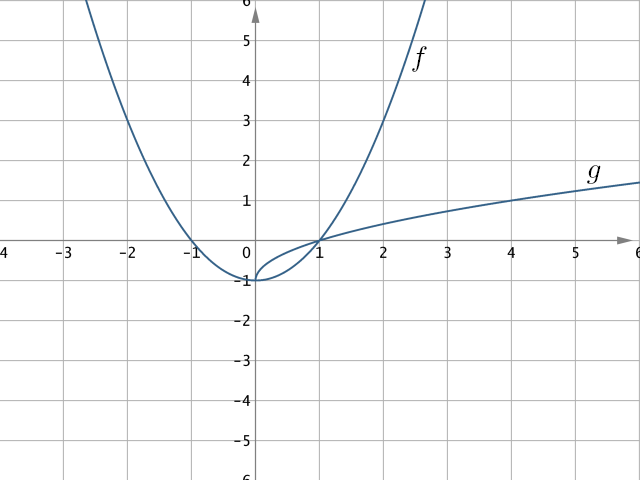
\includegraphics[width=0.5\textwidth]{img/Aufgaben/Analytisch/A1.PNG}
					\end{center}
	\item Aufgabe:
					\[f : \sqrt{\frac 1 2 x^3 \ + \ 2x^2 \ + \ \frac {21} 8 x \ + \ \frac 9 8} \ < \ \sqrt{\frac 1 2 x^2 \ + \ \frac 3 2 x \ + \ \frac 9 8 } \]
				Zwischenschritte: 
	  			\[ \sqrt{ (\frac 1 {\sqrt 2} x \ + \ \frac 3 {\sqrt 2})^2 ( x \ + \ 1)} \ < \ \frac 3 2 \sqrt{(\frac 1	{\sqrt 2} x \ + \ \frac 3 {\sqrt 2})^2}\]
	  			\[\sqrt {(x \ + \ 1)} \ < \ \frac 3 2\]
	  		L\"osung:
	  			\[0 \ < x \ < \ \frac 5 4\]
	  			\begin{center}
						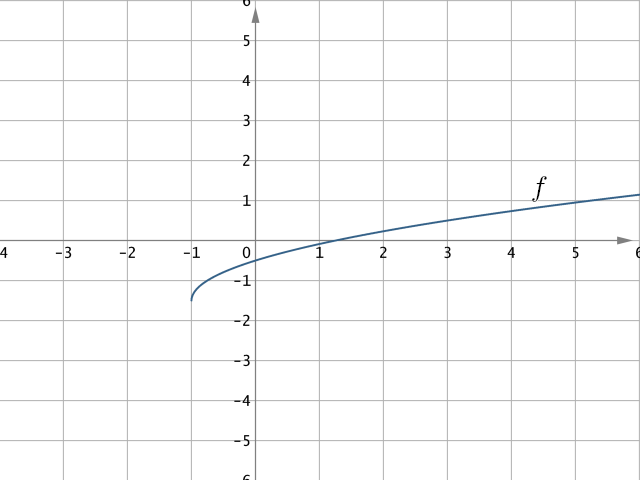
\includegraphics[width=0.5\textwidth]{img/Aufgaben/Analytisch/A2.PNG}
					\end{center}
	\item Aufgabe:
					\[f : \frac 1 2 x^2 \ - \ 1 \ > \ 0\]
				L\"osung:
					\[x \ < \ \sqrt 2 \ \cup \ x \ > \ \sqrt 2\]
					\begin{center}
						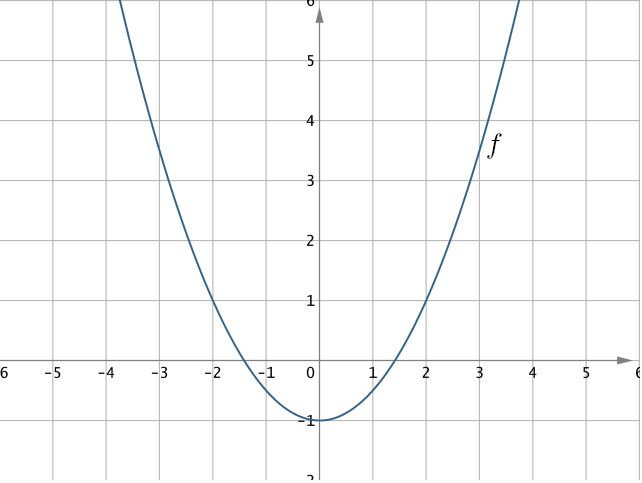
\includegraphics[width=0.5\textwidth]{img/Aufgaben/Analytisch/A3.PNG}
					\end{center}
	\item Aufgabe:
					\[f : x^3 \ + \ 3x^2 \ - \ 4 \ > \ 0\]
				Zwischenschritt:
					\[(x \ - \ 1)(x \ + \ 2)^2 \ > \ 0\]
				L\"osung:	
					\[1 \ < \ x\]
					\begin{center}
						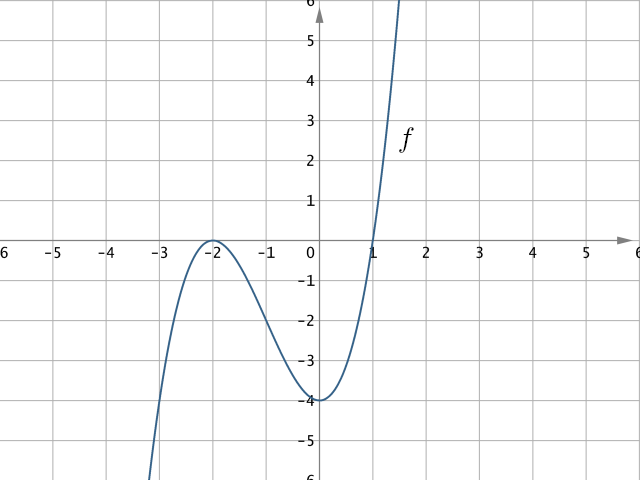
\includegraphics[width=0.5\textwidth]{img/Aufgaben/Analytisch/A4.PNG}
					\end{center}
	\item Aufgabe:
					\[f : x^3 \ + \ 3x^2 \ + \ 3x \ + \ 1 < 0\]
				Tipp: Pascallsches Dreieck \\
				Zwischenschritt:
					\[(x \ + \ 1)^3 < 0\]
				L\"osung:
					\[x \ < \ -1\]
					\begin{center}
						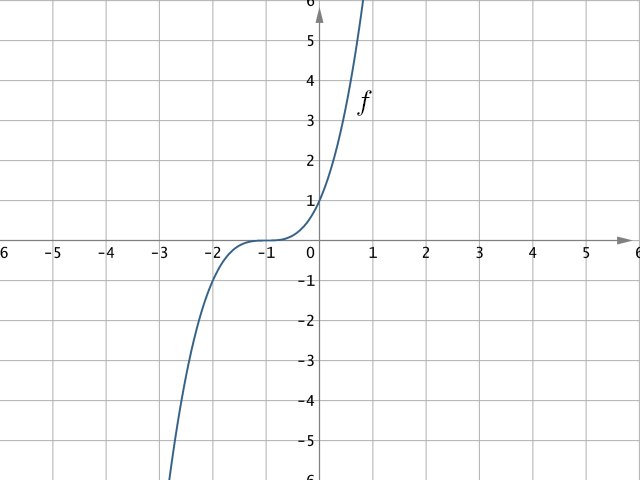
\includegraphics[width=0.5\textwidth]{img/Aufgaben/Analytisch/A5.PNG}
					\end{center}
	\item Aufgabe:
					\[f : x^6 \ - \ 6x^5 \ + \ 15x^4 \ - \ 20x^3 \ + \ 15x^2 \ - \ 6x \ + \ 1 \ \leq \ 0\]
				Nochmal: Pascallsches Dreieck \\
				Zwischenschritt:
					\[(x \ - \ 1)^6 \ \leq \ 0\]
				L\"osung:
					\[x \ \geq \ 1\]
					\begin{center}
						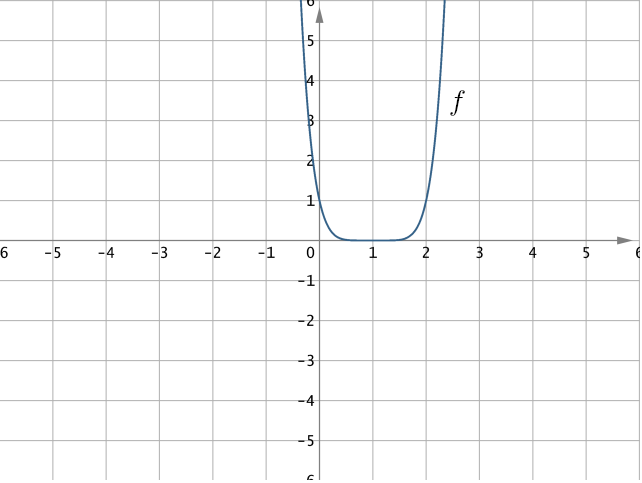
\includegraphics[width=0.5\textwidth]{img/Aufgaben/Analytisch/A6.PNG}
					\end{center}
	\item Aufgabe:
					\[f : \frac 1 2 x^2 \ - \ 8 \ > \ 0\]
					\[g : -3(x \ - \ 1)^2 \ + \ 12 \ > \ 0\]
				L\"osung: \\
					1.Gl: $ x^2 \ > \ 16 \rightarrow x \ > \ 4 \ \cup \ x \ < \ -4 $ \\
					2.Gl: $ -1 \ < \ x \ < \ 3 $ \\
	 				keine L\"osung!
	 				\begin{center}
						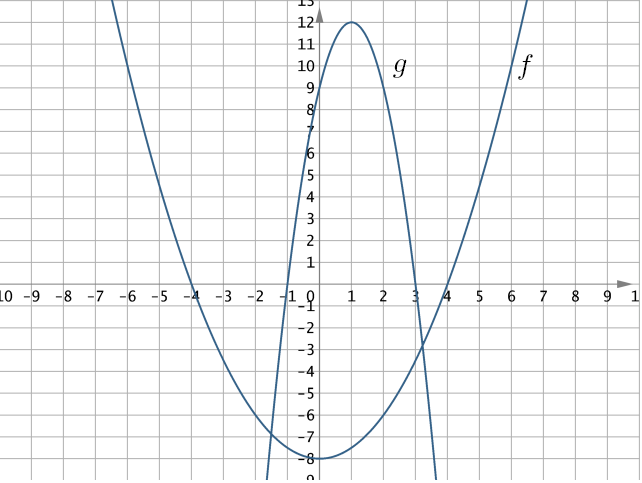
\includegraphics[width=0.5\textwidth]{img/Aufgaben/Analytisch/A7.PNG}
					\end{center}
	\item Aufgabe:
					\[f : (x^2 \ - \ 2)(x \ + \ 1) \ \geq \ 0\]
				L\"osung:
					\[ - \sqrt 2 \ < \ x \ < \ -1 \ \cup \ x \ > \ \sqrt 2\]
					\begin{center}
						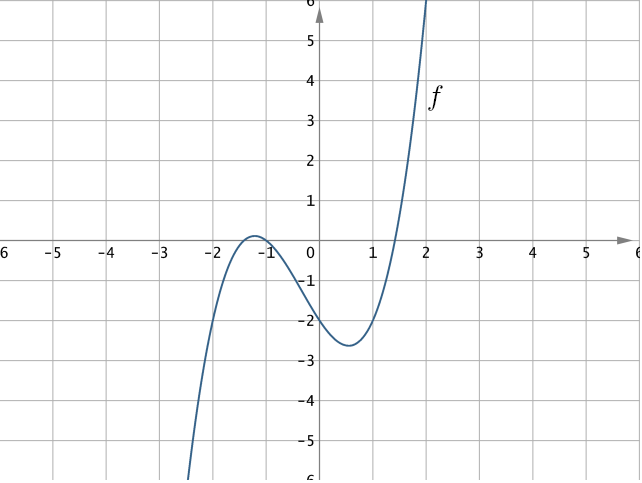
\includegraphics[width=0.5\textwidth]{img/Aufgaben/Analytisch/A8.PNG}
					\end{center}
	\item Aufgabe:
					\[f : ax^2 \ > \ 0\]
					\[g : \frac 1 2 x \ + \ 1 > 0\]
				L\"osung: \\
					1.Gl: $ x \in \mathbb{R} \setminus \lbrace 0 \rbrace $ \\
					2.Gl: $ x \ > \ -2 $
					\[x \ > \ -2 \ und \ x \ \neq \ 0\]
					\begin{center}
						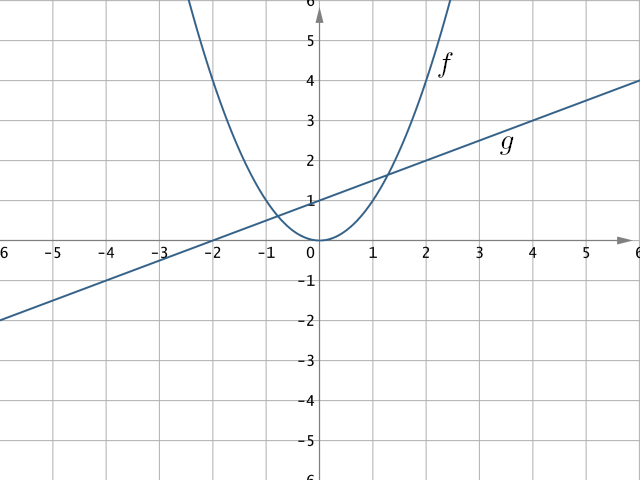
\includegraphics[width=0.5\textwidth]{img/Aufgaben/Analytisch/A9.PNG}
					\end{center}
	\item Aufgabe:
					\[f : x^2 \ + \ a \ > \ 0\]
					\[g : \frac 1 2 x \ + \ 1 \ > \ 0\]
				L\"osung: \\
					1.Gl: \\
						\begin{tabular}{|l|l|}
							\hline $ x \in \mathbb{R} $ & $ a \ > \ 0 $ \\
							\hline $ x \in \mathbb{R} \setminus \lbrace 0 \rbrace $ & $ a \ = \ 0 $ \\
							\hline $ x \ < \ -\sqrt a \ \cup \ x \ > \ \sqrt a \ \  $ & $ a \ < \ 0 $ \\
							\hline
						\end{tabular} \\
					2.Gl: $ x \ > \ -2 $ \\
					\begin{center}
					\begin{tabular}{|l|l|}
						\hline $ x \ > \ -2 $ & $ a \ > \ 0 $ \\
						\hline $ x \ > \ -2 \ $ und $ \ x \ \neq \ 0 $ & $ a \ = \ 0 $ \\
						\hline $ -2 \ < \ x \ < \ -\sqrt a \ \cup \ x \ > \ \sqrt a $ & $ -4 \ < \ a \ < \ 0 $ \\
						\hline $ x \ > \ \sqrt a $ & $ a \ \leq \ -4 $ \\
						\hline
					\end{tabular}
					\end{center}
					\begin{center}
						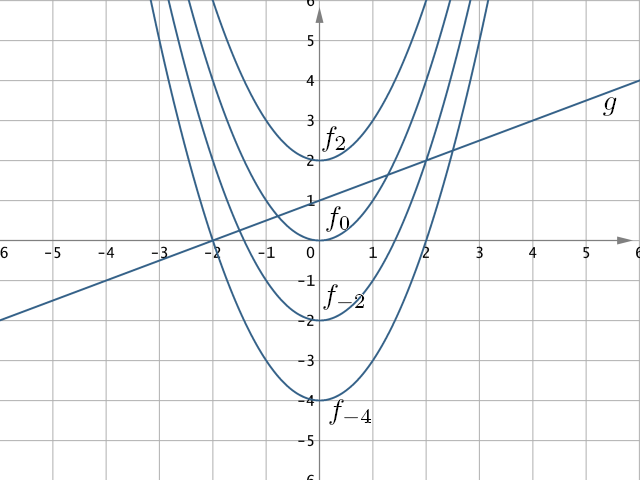
\includegraphics[width=0.5\textwidth]{img/Aufgaben/Analytisch/A10.PNG}
					\end{center}
	\item Aufgabe:
					\[f : -x^2 \ + \ a \ < \ 0\]
					\[g : x \ + \ a \ < \ 0\]
				L\"osung: \\
					1.Gl: \\
						\begin{tabular}{|l|l|}
							\hline $ x \ < \ -\sqrt a \ \cup \ x \ > \sqrt a $ & $ a \ > \ 0 $ \\
							\hline $ x \in \mathbb{R} \setminus \lbrace 0 \rbrace $ & $ a \ = \ 0 $ \\
							\hline $ x \in \mathbb{R} $ & $ a \ < \ 0 $ \\
							\hline
						\end{tabular} \\
					2.Gl: $ x \ < \ -a $
					\begin{center}
					\begin{tabular}{|l|l|}
						\hline $ x \ < \ -a $ & $ a \ > 1 $ \\
						\hline $ x \ < \ -\sqrt a $ & $ 0 \ < \ a \ <= \ 1 $ \\
						\hline $ x \ < \ 0 $ & $ a \ = \ 0 $ \\
						\hline $ x \ < \ -a $ & $ a \ < \ 0 $ \\
						\hline
					\end{tabular}
					\end{center}
					\begin{center}
						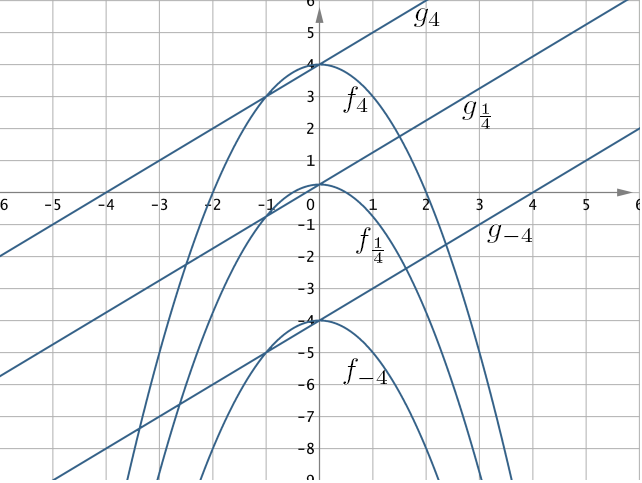
\includegraphics[width=0.5\textwidth]{img/Aufgaben/Analytisch/A11.PNG}
					\end{center}
	\item Aufgabe: 
					\[f : 4x^2 \ - \ 2ax \ + \ \frac 1 4 a^2 \ \geq \ 0\]
				Zwischenschritt:
					\[(x \ - \ \frac 1 4 a)^2 \ \geq \ 0\]
				L\"osung:
					\[x \in \mathbb{R} \setminus \lbrace \frac 1 4 a \rbrace\]
					\begin{center}
						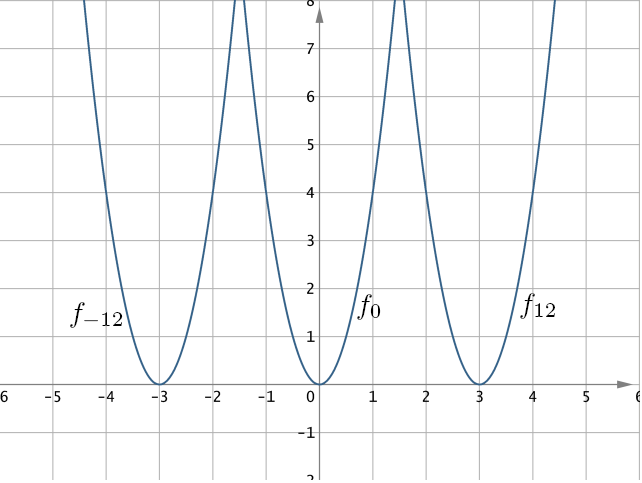
\includegraphics[width=0.5\textwidth]{img/Aufgaben/Analytisch/A12.PNG}
					\end{center}
	\item Aufgabe:
					\[f : x^3 \ + \ x^2 \ - \ 2x \ \geq \ 2\]
					(siehe Aufgabe 8) \\
				L\"osung:
					\[ - \sqrt 2 \ < \ x \ < \ -1 \ \cup \ x \ > \ \sqrt 2\]
					\begin{center}
						\includegraphics[width=0.5\textwidth]{img/Aufgaben/Analytisch/A13.PNG}
					\end{center}
	\item Aufgabe:
					\[f : (x \ - \ 1)^2 \ - \ 4 \ < \ 0\]
					\[g : -(x \ + \ 1)^2 \ + \ 4 \ > \ 0\]
				L\"osung: \\
					1.Gl: $ -1 \ < \ x \ < \ 3 $ \\
					2.Gl: $ -3 \ < \ x \ < \ 1 $ \\
					\[-1 \ < \ x \ < \ 1\]
					\begin{center}
						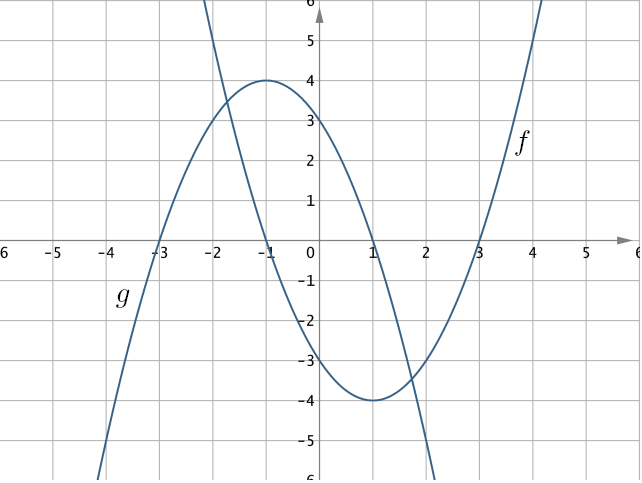
\includegraphics[width=0.5\textwidth]{img/Aufgaben/Analytisch/A14.PNG}
					\end{center}
	\item Aufgabe:
					\[f : \sqrt {(x-1)} \ \geq \ 0\]
					\[g : - \frac 1 4 x \ + \ 4 \ < \ 0\]
				L\"osung: \\
					1.Gl: $ x \ \geq \ 1 $ \\
					2.Gl: $ x \ > \ 16 $
					\[ x \ > \ 16\]
					\begin{center}
						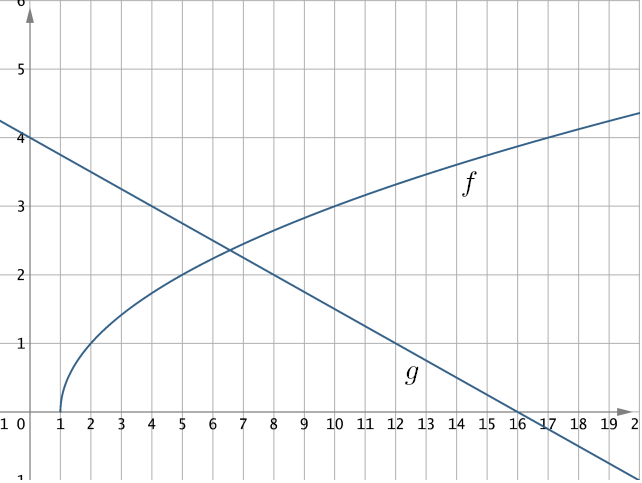
\includegraphics[width=0.5\textwidth]{img/Aufgaben/Analytisch/A15.PNG}
					\end{center}
	\item Aufgabe:
					\[f : x^4 \ - \ 16 \ \leq \ 0\]
					\[g : x^3 \ + \ 1 \ \geq \ 0\]
				L\"osung: \\
					1.Gl: $ -2 \ \leq \ x \ \leq \ 2 $ \\
					2.Gl: $ x  \ \geq \ -1 $ \\
					\[-1 \ \leq \ x \ \leq \ 2\]
					\begin{center}
						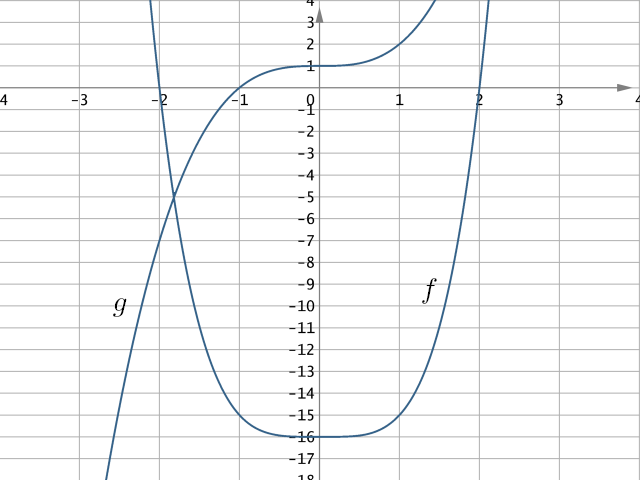
\includegraphics[width=0.5\textwidth]{img/Aufgaben/Analytisch/A16.PNG}
					\end{center}
\end{enumerate}

\subsection{Ungleichungen mit mehreren Variablen}

\begin{enumerate}
	\item Aufgabe: 
					\[f : x^2 \ + \ y^2 \ < \ 25 \]
					\[g : \frac 1 2 x \ + \ \frac 5 2 \ > \ y \]
					\[h : -x \ - \ 5 \ < \ y \]
				L\"osung:
				\begin{center}
						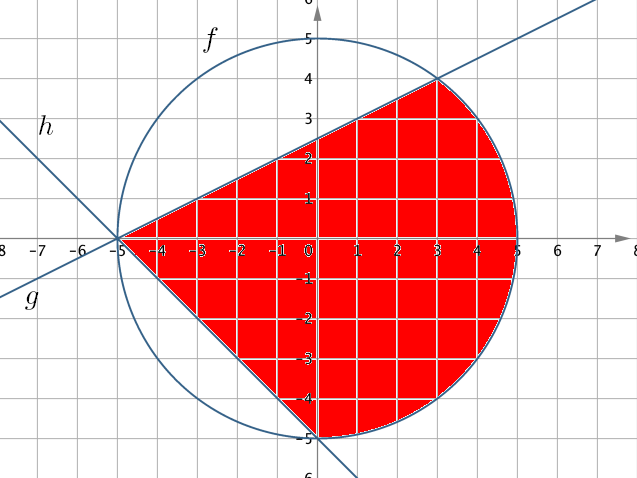
\includegraphics[width=0.5\textwidth]{img/Aufgaben/Graphisch/A1.PNG}
				\end{center}
	\item Aufgabe:
					\[f : - x^2 \ + \ 5 \ < \ y \]
					\[g : x(x \ - \ 3)^2 \ > \ y \]
					\[h : -x \ - \ 2 \ > \ y \]
				L\"osung:
					\begin{center}
						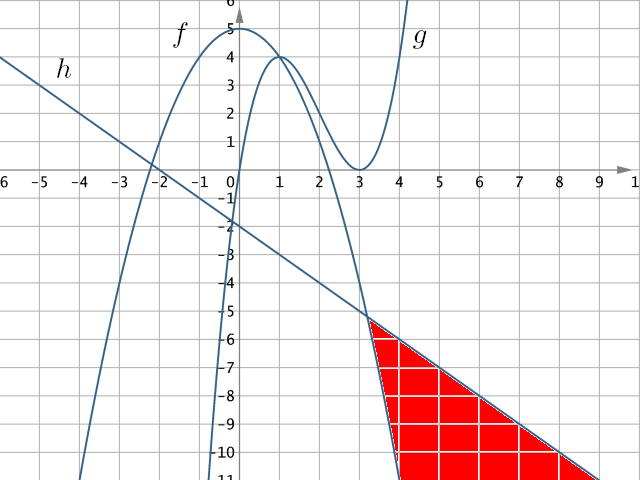
\includegraphics[width=0.5\textwidth]{img/Aufgaben/Graphisch/A2.PNG}
					\end{center}
	\item Aufgabe:
					\[f : 3x^2 \ - \ 3x \ - \ 10 \ < \ -4 \ + \ y \]
					\[g : y \ \leq \ \frac 1 2 \]
				L\"osung:
					\begin{center}
						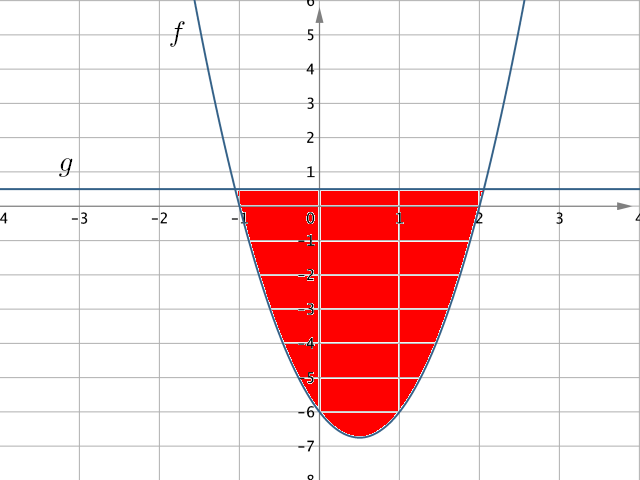
\includegraphics[width=0.5\textwidth]{img/Aufgaben/Graphisch/A3.PNG}
					\end{center}
	\item Aufgabe:
					\[f : y \ < \ \frac {2x^2 \ + \ 3x \ + \ 4} {- x^4 \ - \ 2x^3 \ - \ x^2 \ + \ 4x \ + \ (2x \ + \ x^2)^2} \]
					\[g : - \frac 1 x \ < \ y \]
					\[h : - ( \frac 1 {\sqrt 2} x )^2 \ < \ y \ - \ \frac 1 2 x^2 \ + \ \frac 1 2 x \ + \ 2 \]
					\[i : y \ + \ x \ - \ 2 \ < \ 0 \]
				Zwischenschritt:
				\[f : y \ < \ \frac 1 x\]
				\[h : y \ > \ -\frac 1 2 x \ - \ 2\]
				L\"osung:
					\begin{center}
						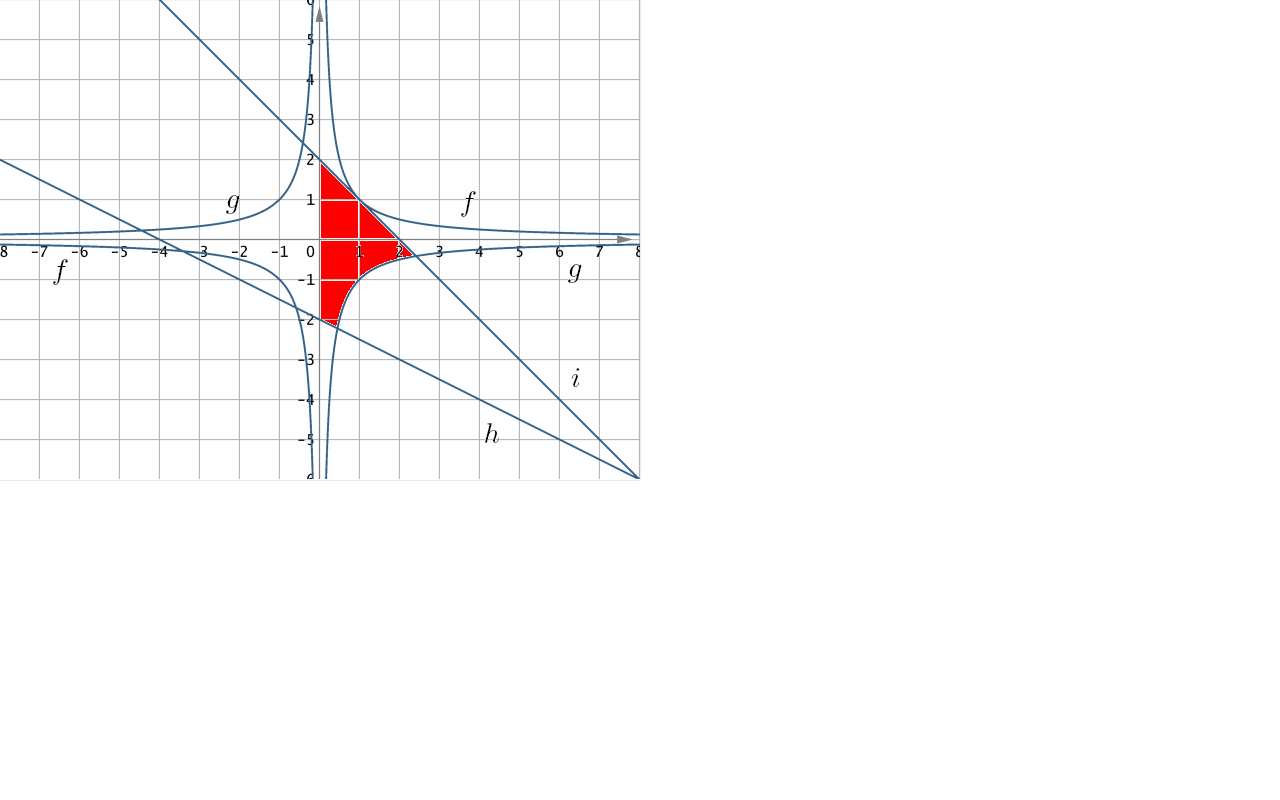
\includegraphics[width=0.5\textwidth]{img/Aufgaben/Graphisch/A4.PNG}
					\end{center}
	\item Aufgabe:
					\[f : \frac 1 2 x^2 \ - \ 3x \ \leq \ y\]
					%\[g : \frac 4x^3 \ + \ 2x^2 \ - \ \frac {13} 4 x \ \geq \ y\]
					\[g : y \ \leq \ -x\]
					\[h : 17x^3 \ - \ \frac 1 2 \ = \ y\]
				L\"osung:
					\begin{center}
						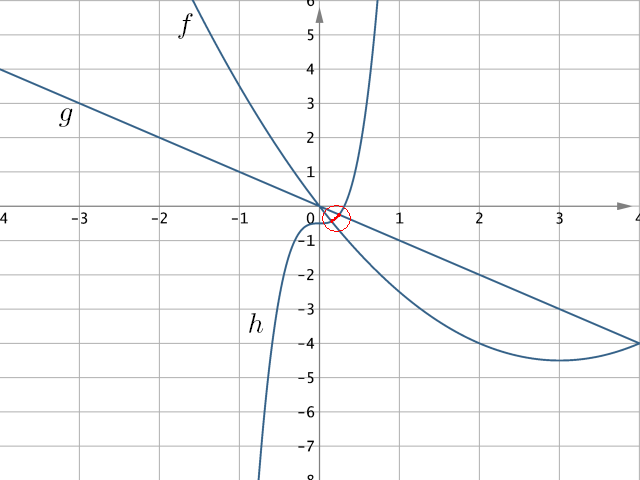
\includegraphics[width=0.5\textwidth]{img/Aufgaben/Graphisch/A5.PNG}
					\end{center}
	\item Aufgabe:
					\[f : y \ + \ \sqrt {\frac {x^3 \ + \ x^2 \ - \ x \ - \ 1} {x \ - \ 1}} \ > \ 0 \]
					\[g : \frac 2 {20} x \ - \ \frac 1 3 y \ + \ \frac 3 {12} \ < \ 0\]
				Zwischenschritt:
				\[f : y \ > \ -x \ - \ 1\]
				\[g : y \ > \ \frac {10} 3 x \ + \ \frac 3 4\]
				L\"osung:
					\begin{center}
						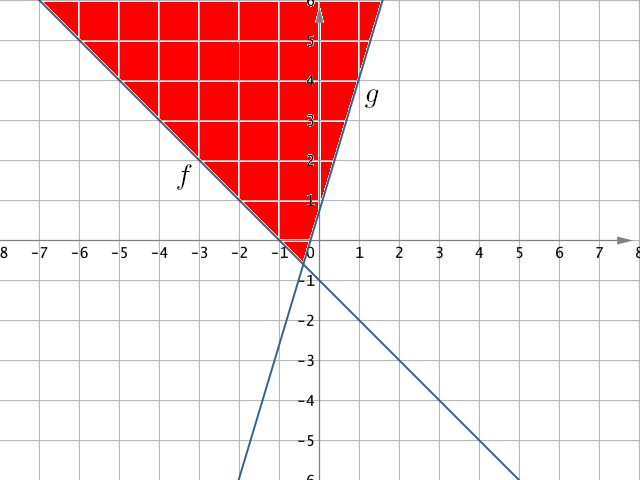
\includegraphics[width=0.5\textwidth]{img/Aufgaben/Graphisch/A6.PNG}
					\end{center}
	\item Aufgabe:
					\[f : \frac 1 2 x \ - \ 2 < y\]
					\[g : \frac 1 2 x \ + \ 2 > y\]
					\[h : 2 x \ - \ 4 < y\]
					\[i : 2 x \ + \ 4 > y\]
					\[k : - \frac 1 2 x \ - \ 2 < y\]
					\[l : - \frac 1 2 x \ + \ 2 > y\]
					\[m : -2 x \ - \ 4 < y\]
					\[n : -2 x \ + \ 4 > y\]
				L\"osung:
					\begin{center}
						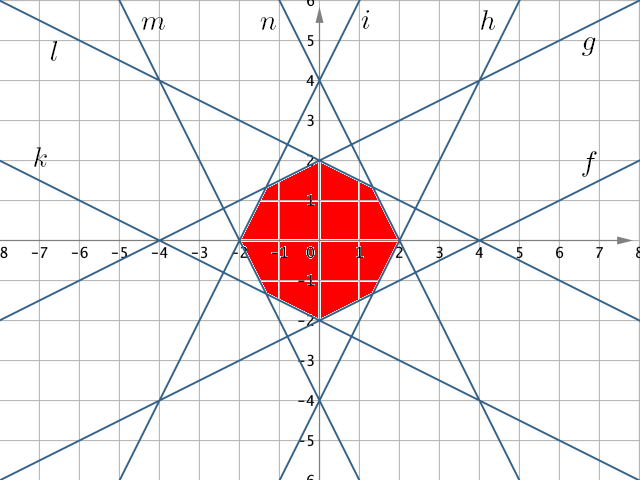
\includegraphics[width=0.5\textwidth]{img/Aufgaben/Graphisch/A7.PNG}
					\end{center}
	\item Aufgabe:
					\[f : |(x^2 \ + \ (y \ - \ 1)^2| \ = \ 4 \]
					\[g : x \ \geq \ y \]
				L\"osung:
					\begin{center}
						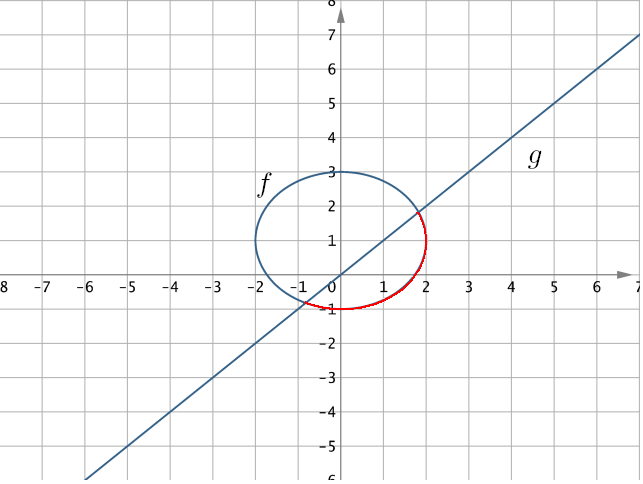
\includegraphics[width=0.5\textwidth]{img/Aufgaben/Graphisch/A8.PNG}
					\end{center}
	\item Aufgabe:
					\[f : ((\sin x) \ + \ \frac 1 2)^2 \ - \ \frac 3 4 \ - \ y \ - \ (\sin x)^2 < 0\]
					\[g : \cos (x \ + \ \frac {\pi} 2 ) + \ \frac 1 2 \ < \ y \]
				Zwischenschritt:
					\[f : y \ < \ \sin x \ - \ \frac 1 2\]
				L\"osung:
					\begin{center}
						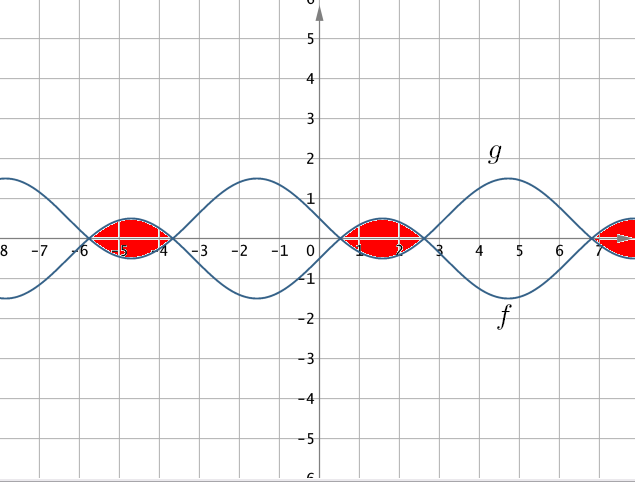
\includegraphics[width=0.5\textwidth]{img/Aufgaben/Graphisch/A9.PNG}
					\end{center}
	\item Aufgabe:
					\[f : |\frac 1 x| \ > y \]
					\[g : - \frac {1 \ + \ 7x^2} {x^2 y} > \ - \frac {y \ + \ 7} y\]
					\[h : |x| + y < 5\]
				Zwischenschritt:
					\[g : y \ > \ \frac 1 {x^2}\]
				L\"osung:
					\begin{center}
						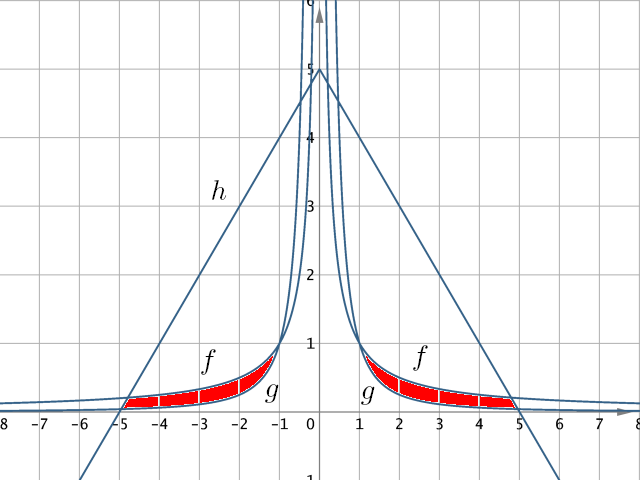
\includegraphics[width=0.5\textwidth]{img/Aufgaben/Graphisch/A10.PNG}
					\end{center}
	\item Aufgabe:
					\[f : 4x^2 \ + \ y^2 \ <= \ 16\]
					\[g : x^2 \ + \ 4y^2 \ <= \ 16\]
				L\"osung:
					\begin{center}
						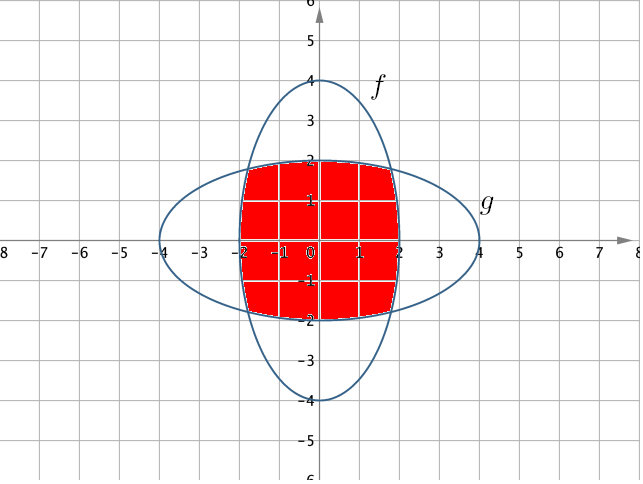
\includegraphics[width=0.5\textwidth]{img/Aufgaben/Graphisch/A11.PNG}
					\end{center}
	\item Aufgabe:
					\[f : (y \ - \ 2)^2 \ < \ 4 - (x \ - \ 2)^2\]
					\[g : y -2 < 0\]
					\[h : -|x \ - \ 2| \ + \ 2\ < \ y\]
				L\"osung:
					\begin{center}
						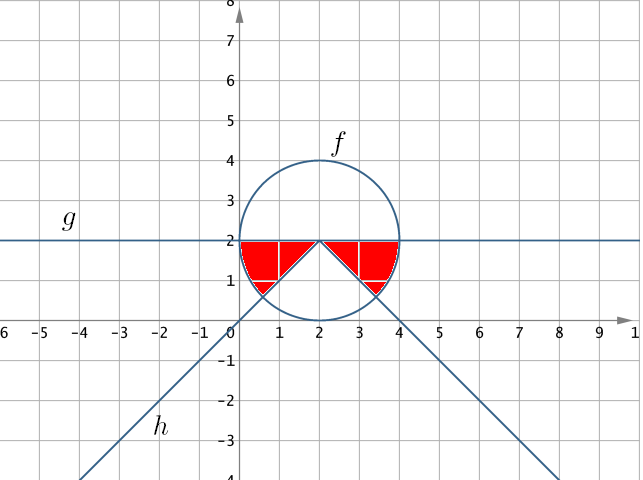
\includegraphics[width=0.5\textwidth]{img/Aufgaben/Graphisch/A12.PNG}
					\end{center}
	\item Berechnen Sie f\"ur die Ungleichung den Fl\"acheninhalt der L\"osungsmenge! \\
				Aufgabe:
					\[f : (2y \ - \ 3)^2 \ + \ (3y \ + \ 2)^2 \ + \ y \ - \ 10 \ \geq \ | \frac {4x \ + \ 4 (\frac 1 2 x \ - \frac 3 2 )^2 \ - \ 9} x | \ + \ 13y^2 \]
					\[g : y \ \leq \ -1\]
				Zwischenschritt:
					\[f : y \ \geq \ |x-2|-3\]
				L\"osung: Fl\"acheninhalt $ = \ 4 $
					\begin{center}
						\includegraphics[width=0.5\textwidth]{img/Aufgaben/Fl\"acheninhalt/A13.PNG}
					\end{center}
	\item Berechnen Sie f\"ur das Ungleichungssystem den Fl\"acheninhalt der L\"osungsmenge! \\
				Aufgabe:
					\[f : x^2 \ - \ 4x \ + 4 \ + \ y^2 \ - \ 2y \ + \ 1 \ \geq \ 1 \]
					\[g : (x \ - \ 2)^2 \ + \ (y \ - \ 2)^2 \ \leq \ 4 \]
					\[h : (x \ - \ 2)^2 \ + \ (y \ - \ 3)^2 \ \geq \ 1 \]
				Zwischenschritt:
					\[f : (x \ - \ 2)^2 + (y \ - \ 1)^2 \ \geq \ 1\]
				L\"osung: Fl\"acheninhalt $ = 4 \pi \ - \ 2 \pi \ = 2 \pi $
					\begin{center}
						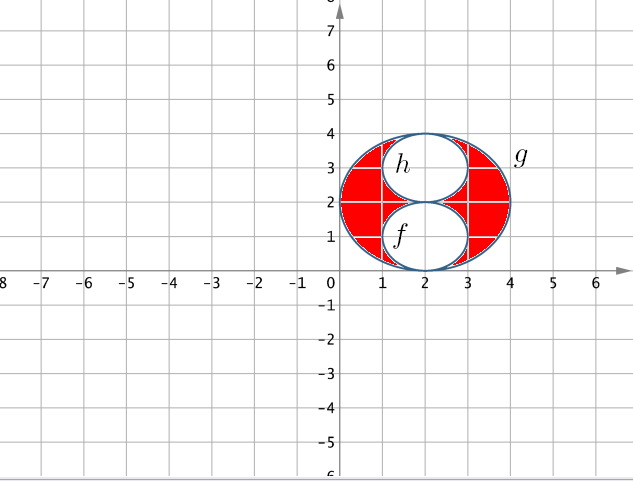
\includegraphics[width=0.5\textwidth]{img/Aufgaben/Fl\"acheninhalt/A14.PNG}
					\end{center}
	\item F\"ur welches a ist der Fl\"acheninhalt der L\"osungsmenge $ = 2 $ ?
				Aufgabe:
					\[f : y \ \geq \ 2\]
					\[g : -|x| \ + \ a \ \leq \ y\]
				L\"osung: Fl\"acheninhalt $ = 2 $ f\"ur $ a = 2 $
					\begin{center}
						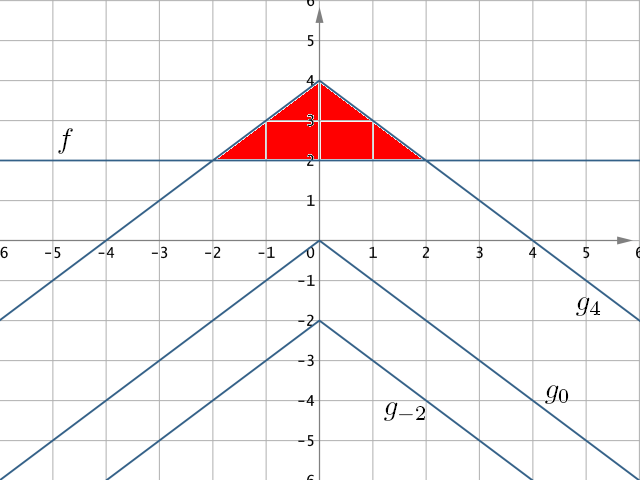
\includegraphics[width=0.5\textwidth]{img/Aufgaben/Fl\"acheninhalt/A15.PNG}
					\end{center}
	\item Bestimmen Sie ein $a$ und ein $ b $, f\"ur das der Fl\"acheninhalt der L\"osungsmenge $ 2 \pi $ ergibt! \\
				Aufgabe:
					\[f : - \frac 1 3 x \ \leq y \ - \ 2\]
					\[g : (x+ \frac 1 4 b)^2 \ + \ (y \ - \ \frac 3 2 a)^2 \ \leq \ a^2\]
				(einfachste) L\"osung: $ a = 2 $ , $ b = 12 $
					\begin{center}
						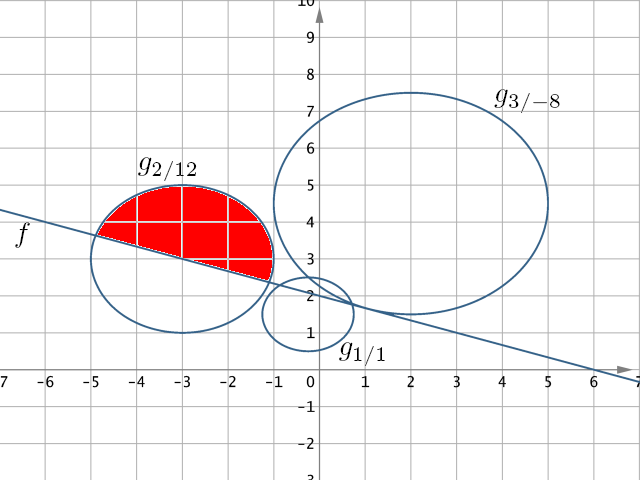
\includegraphics[width=0.5\textwidth]{img/Aufgaben/Fl\"acheninhalt/A16.PNG}
					\end{center}
	\item Beschreiben sie die L\"osungsmenge des Ungleichungssystems! \\
				Aufgabe:
					\[f : x^2 \ + \ y^2 \ + \ z (z \ + \ 2) \ < \ 8 \]
					\[g : x \ \leq \ 0 \]
					\[h : y \ \leq \ 0 \]
				Zwischenschritt:
					\[f : x^2 \ + \ y^2 \ + \ (z \ + \ 1)^2 \ < \ 9\]
				L\"osung: \\
				Die L\"osungsmenge ist eine Halbkugel unter der x-y-Ebene im $ \mathbb{R}^3 $, die um eine Einheit in z-Richtung verschoben ist.
	\item Beschreiben sie die L\"osungsmenge des Ungleichungssystems! \\
				Aufgabe:
					\[f : (x \ - \ 2 \sqrt 3)^2 \ + \ (x \ - \ 2 \sqrt 3)^2 \ + \ (z \ - \ 2 \sqrt 3)^2 \ \leq \ 36\]
					\[g : (x \ + \ 2 \sqrt 3)^2 \ + \ (x \ + \ 2 \sqrt 3)^2 \ + \ (z \ + \ 2 \sqrt 3)^2 \ \leq \ 36\]
				L\"osung: \\
				Es ist schnell ersichtlich, dass es sich mit zwei Kugeln mit Radius $ r = 6 $ handelt. 
				Bei n\"aherer Betrachtung ist zu erkennen, dass der Abstand des Mittelpunktes ebenfalls 6 betr\"agt.
				Da sich die Kugeln genau gegen\"uberliegen, haben sie nur den Ursprung als gemeinsame L\"osung.
				Die L\"osungsmenge ist somit nur der Punkt mit $ x = 0, y = 0, z = 0 $.
\end{enumerate}

% BEtrag ungleichunge kreis
%\chapter{Vollständige Induktion Lösung}
Autor: Katja Matthes
\section{Gleichungen}
\subsubsection{Aufgabe 1}
\textbf{Gesucht:} Formeln für $ 1 + 3 + 5 + ... + 2n-1 = \sum_{k=1}^n 2k-1 $ \\
\textbf{Finden der Vermutung:}\begin{align*} 	\sum_{k=1}^1 2k-1 &= 1 &\quad \sum_{k=1}^3 2k-1 &= 9 \\
																							\sum_{k=1}^2 2k-1 &= 4 &\quad \sum_{k=1}^4 2k-1 &= 16	\end{align*}\\
\textbf{Zu Zeigen}: \quad							$\sum_{k=1}^n 2k-1 = n^2 $ \\
\textbf{Ind.anfang}: \quad$n_0 = 1$ \\
\textbf{Ind.voraussetzung}:\quad $\sum_{k=1}^n 2k-1 = n^2$ \\
\textbf{Ind.behauptung}:\quad$ \sum_{k=1}^{n+1} 2k-1 = (n+1)^2$ \\
\textbf{Induktionsbeweis}: \begin{align*}
	\sum_{k=1}^{n+1} 2k-1 &= \sum_{k=1}^n 2k-1 + 2(n+1)-1 && \text{\textbar nach Voraussetzung}\\
												&= n^2 + 2n+2-1 								&& \text{\textbar Zusammenfassen}\\
												&= n^2 + 2n + 1 								&& \text{\textbar Binomische Formel}\\
												&= (n+1)												&& \text{\textbar qed}\end{align*}
%%%%%%%%%%%%%%%%%%%%%%%%%%%%%%%%%%%%%%%%%%%%%%%%%%%%%%%%%%%%%%%%%%%%%%%%%%%%%%%%%%%%%%%%%%%%%%%%%%%%%%%%%%%%%
\subsubsection{Aufgabe 2}
\textbf{Gesucht:} Formeln für $ 4 + 8 + 12 + ... + 4n = 2n(n+1) = \sum_{k=1}^n 4k$ \\
\textbf{Finden der Vermutung:}\begin{align*} 	\sum_{k=1}^1 4k = 4  &= 2\cdot1\cdot2 &\sum_{k=1}^3 4k = 24 &= 2\cdot3\cdot4\\
																							\sum_{k=1}^2 4k = 12 &= 2\cdot2\cdot3 &\sum_{k=1}^4 4k = 40 &= 2\cdot4\cdot5 \end{align*}\\
\textbf{Zu Zeigen}:\quad$\sum_{k=1}^n 4k = 2n(n+1) $ \\
\textbf{I.anfang}:\quad$ n_0 = 1$ \\
\textbf{I.voraussetzung}:\quad$\sum_{k=1}^n 4k = 2n(n+1) $\\
\textbf{I.behauptung}: \quad $\sum_{k=1}^{n+1} 4k = 2(n+1)((n+1)+1) $\\
\textbf{Induktionsbeweis}: \begin{align*}
	\sum_{k=1}^{n+1} 4k &= \sum_{k=1}^n 4k + 4(n+1)	&& \text{\textbar Voraussetzung}\\
											&= 2n(n+1) + 4(n+1)					&& \text{\textbar $2$ Ausklammern}\\
											&= 2(n(n+1)+2(n+1))					&& \text{\textbar $(n+1)$ Ausklammern}\\
											&= 2(n+1)(n+2)							&& \\
											&= 2(n+1)((n+1)+1)				&& \text{\textbar qed}\end{align*}
%%%%%%%%%%%%%%%%%%%%%%%%%%%%%%%%%%%%%%%%%%%%%%%%%%%%%%%%%%%%%%%%%%%%%%%%%%%%%%%%%%%%%%%%%%%%%%%%%%%%%%%%%%%%%%%%
\subsubsection{Aufgabe 3}
\textbf{I.anf.}:\quad$ n_0 = 1 \Rightarrow \sum_{k=1}^1 2k = 2\cdot1 = 2 = 1^2+1$ \\
\textbf{I.vor.}: \quad$\sum_{k=1}^{n} 2k = n^2 + n $\\
\textbf{I.beh.}:\quad$\sum_{k=1}^{n+1} 2k = (n+1)^2 + (n+1) $\\
\textbf{Induktionsbeweis}:  \begin{align*} 
		\sum_{k=1}^{n+1} 2k 	&= \sum_{k=1}^{n} 2k + 2(n+1) && \text{\textbar Voraussetzung}\\
													&= n^2 + n + 2(n+1) 					&& \text{\textbar Ausmultiplizieren}\\
													&= n^2 + n + 2n + 2						&& \text{\textbar Umordnen}\\
													&= n^2 + 2n + 1 + n+1 				&& \text{\textbar Binomische Formel}\\
													&= (n+1)^2 + (n+1) 						&& \text{\textbar qed}\end{align*}
%%%%%%%%%%%%%%%%%%%%%%%%%%%%%%%%%%%%%%%%%%%%%%%%%%%%%%%%%%%%%%%%%%%%%%%%%%%%%%%%%%%%%%%%%%%%%%%%%%%%%%%%%%%%
\subsubsection{Aufgabe 4}
\textbf{I.anf.}:\quad $n_0 = 1 \Rightarrow \sum^1_{k=1} \frac{1}{(2k-1)(2k+1)} = \frac{1}{3}= \frac{1}{2\cdot1+1}$\\
\textbf{I.vor.}:\quad$\sum^n_{k=1} \frac{1}{(2k-1)(2k+1)} = \frac{n}{2n + 1}$ \\
\textbf{I.beh.}:\quad$\sum^{n+1}_{k=1} \frac{1}{(2k-1)(2k+1)} = \frac{n+1}{2(n+1) + 1} $\\
\textbf{Induktionsbeweis}: \begin{align*}
&\sum^{n+1}_{k=1} \frac{1}{(2k-1)(2k+1)}\\ 
= &\sum^n_{k=1} \frac{1}{(2k-1)(2k+1)} + \frac{1}{(2(n+1)-1)(2(n+1)+1)} \\
& \qquad\text{\textbar Voraussetzung}\end{align*}\begin{align*}
																				= &\frac{n}{2n + 1} + \frac{1}{(2n+1)(2n+3)} && \\
																				= &\frac{n \cdot (2n+3) + 1}{(2n+1)(2n+3)} 		&& \text{\textbar Ausmultiplizieren}\\
																				= &\frac{2n^2 + 3n + 1}{(2n+1)(2n+3)} 				&& \text{\textbar Polynomdivision}\\
																				= &\frac{(2n+1)(n+1)}{(2n+1)(2n+3)} 					&& \text{\textbar Kürzen}\\
																				= &\frac{n+1}{2n+3}														&& \text{\textbar Umformen}\\
																				= &\frac{n+1}{2(n+1) + 1} 										&& \text{\textbar qed}
\end{align*}
%%%%%%%%%%%%%%%%%%%%%%%%%%%%%%%%%%%%%%%%%%%%%%%%%%%%%%%%%%%%%%%%%%%%%%%%%%%%%%%%%%%%%%%%%%%%%%%%%%%%%%%%%%
\subsubsection{Aufgabe 5}
\textbf{I.anf.}:\quad$n_0 = 1 \Rightarrow \sum^1_{k=1} \frac{1}{k(k+1)} = \frac{1}{2} = \frac{1}{1+1}$\\
\textbf{I.vor.}: \quad$\sum^n_{k=1} \frac{1}{k(k+1)} = \frac{n}{n+1} $\\
\textbf{I.beh.}:\quad$\sum^{n+1}_{k=1} \frac{1}{k(k+1)} = \frac{n+1}{(n+1)+1} $\\
\textbf{Induktionsbeweis}:\begin{align*} 
&\sum^{n+1}_{k=1} \frac{1}{k(k+1)} \\
= &\sum^n_{k=1} \frac{1}{k(k+1)} + \frac{1}{(n+1)((n+1)+1)} && \text{\textbar Voraussetzung}\\
																	= &\frac{n}{n+1} + \frac{1}{(n+1)(n+2)} \\
																	= &\frac{n \cdot (n+2) +1}{(n+1)(n+2)} && \text{\textbar Ausmultiplizieren}\\
																	= &\frac{n^2 + 2n + 1}{(n+1)(n+2)} && \text{\textbar Binomische Formel}\\
																	= &\frac{(n+1)^2}{(n+1)(n+2)} && \text{\textbar Kürzen}\\
																	= &\frac{n+1}{n+2}						&& \text{\textbar Umformen}\\
																	= &\frac{n+1}{(n+1)+1} 				&& \text{\textbar qed}\end{align*}
%%%%%%%%%%%%%%%%%%%%%%%%%%%%%%%%%%%%%%%%%%%%%%%%%%%%%%%%%%%%%%%%%%%%%%%%%%%%%%%%%%%%%%%%%%%%%%%%%%%%%%%%%%%%
\subsubsection{Aufgabe 6}
\textbf{I.anf.}:\quad$ n_0 = 1 \Rightarrow \sum^1_{k=1} k = 1 = \frac{2}{2} = \frac{1(1+1)}{2}$\\
\textbf{I.vor.}: \quad$\sum^n_{k=1} k = \frac{n(n+1)}{2}$ \\
\textbf{I.beh.}:\quad$\sum^{n+1}_{k=1} k = \frac{(n+1)((n+1)+1)}{2} $\\
\textbf{Induktionsbeweis}: \begin{align*}
\sum^{n+1}_{k=1} k &= \sum^n_{k=1} k + (n+1) && \text{\textbar Voraussetzung}\\
										&= \frac{n(n+1)}{2} + (n+1)\\
										&= \frac{n(n+1) + 2(n+1)}{2} && \text{\textbar $(n+1)$ Ausklammern}\\
										&= \frac{(n+1)(n + 2)}{2} && \text{\textbar Umformen}\\
										&= \frac{(n+1)((n+1)+1)}{2} && \text{\textbar qed} \end{align*}	
%%%%%%%%%%%%%%%%%%%%%%%%%%%%%%%%%%%%%%%%%%%%%%%%%%%%%%%%%%%%%%%%%%%%%%%%%%%%%%%%%%%%%%%%%%%%%%%%%%%%%%%%
\subsubsection{Aufgabe 7}
\textbf{I.anf.}:\quad $n_0 = 1 \Rightarrow \sum_{k=1}^1 k^2 = 1^2 = \frac{6}{6} = \frac{1(1+1)(2\cdot1+1)}{6} $\\
\textbf{I.vor.}:\quad $\sum_{k=1}^n k^2 = \frac{n(n+1)(2n+1)}{6} $ \\
\textbf{I.beh.}: \quad$\sum_{k=1}^{n+1} k^2 = \frac{(n+1)((n+1)+1)(2(n+1)+1)}{6} $\\
\textbf{Induktionsbeweis}: \begin{align*}
\sum_{k=1}^{n+1} k^2 &= \sum_{k=1}^n k^2 + (n+1)^2 && \text{\textbar Voraussetzung}\\
											&= \frac{n(n+1)(2n+1)}{6} + (n+1)^2 \\
											&= \frac{n(n+1)(2n+1) + 6(n+1)^2}{6} && \text{\textbar $(n+1)$ Ausklammern}\\
											&= \frac{(n+1)(n(2n+1) + 6(n+1))}{6} \\
											&= \frac{(n+1)(2n^2 + 7n + 6)}{6} && \text{\textbar Polynomdivision}\\
											&= \frac{(n+1)(n+2)(2n+3)}{6} && \text{\textbar Umformen}\\
											&= \frac{(n+1)((n+1)+1)(2(n+1)+1)}{6} && \text{\textbar qed}\end{align*}	
%%%%%%%%%%%%%%%%%%%%%%%%%%%%%%%%%%%%%%%%%%%%%%%%%%%%%%%%%%%%%%%%%%%%%%%%%%%%%%%%%%%%%%%%%%%%%%%%%%%
\subsubsection{Aufgabe 8}
\textbf{I.anf.}:\quad$ n_0 = 1 \Rightarrow \sum_{k=1}^1 \frac{k}{2^k} = \frac{1}{2^1} = 2 - \frac{3}{2} = 2 - \frac{1+2}{2^1}$\\
\textbf{I.vor.}:\quad$ \sum_{k=1}^n \frac{k}{2^k} = 2 - \frac{n+2}{2^n}$ \\
\textbf{I.beh.}:\quad$ \sum_{k=1}^{n+1} \frac{k}{2^k} = 2 - \frac{(n+1)+2}{2^{n+1}}$ \\
\textbf{Induktionsbeweis}:\begin{align*} 
\sum_{k=1}^{n+1} \frac{k}{2^k} &= \sum_{k=1}^n \frac{k}{2^k} + \frac{n+1}{2^{n+1}} && \text{\textbar Voraussetzung}\\
																&= 2 - \frac{n+2}{2^n} + \frac{n+1}{2^{n+1}} \\
																&= 2 + \frac{-2(n+2)+(n+1)}{2^{n+1}} && \text{\textbar Zusammenfassen}\\
																&= 2 + \frac{-(n+3)}{2^{n+1}} && \text{\textbar $(-)$ Vorziehen}\\
																&= 2 - \frac{(n+1)+2}{2^{n+1}} && \text{\textbar qed} \end{align*}	
%%%%%%%%%%%%%%%%%%%%%%%%%%%%%%%%%%%%%%%%%%%%%%%%%%%%%%%%%%%%%%%%%%%%%%%%%%%%%%%%%%%%%%%%%%%%%%%%%%%
\subsubsection{Aufgabe 9}
\textbf{I.anf.}:\quad$ n_0 = 0 \Rightarrow \sum_{k=0}^0 \left(\frac{2}{3}\right)^k = \frac{2}{3} = 3\cdot \frac{1}{3} = 3\left(1-\frac{2}{3}^{0+1}\right)$\\
\textbf{I.vor.}:\quad$\sum_{k=0}^n \left(\frac{2}{3}\right)^k = 3 \cdot \left(1 - \left(\frac{2}{3}\right)^{n+1}\right)$ \\
\textbf{I.beh.}\quad$ \sum_{k=0}^{n+1} \left(\frac{2}{3}\right)^k = 3 \cdot \left(1 - \left(\frac{2}{3}\right)^{(n+1)+1}\right) $\\
\textbf{Induktionsbeweis}:\begin{align*} 
\sum_{k=0}^{n+1} \left(\frac{2}{3}\right)^k &= \sum_{k=0}^n \left(\frac{2}{3}\right)^k + \left(\frac{2}{3}\right)^{n+1} && \text{\textbar Voraussetzung}\\
																						&= 3 \cdot \left(1 - \left(\frac{2}{3}\right)^{n+1}\right) + \left(\frac{2}{3}\right)^{n+1} && \text{\textbar R. Br. mit $3$ erweitern}\\
																						&= 3 \cdot \left(1 - \left(\frac{2}{3}\right)^{n+1}\right) + \frac{3 \cdot 2^{n+1}}{3^{n+2}} && \text{\textbar $3$ Ausklammern}\\
																						&= 3 \cdot \left(1 - \left(\frac{2}{3}\right)^{n+1} + \frac{2^{n+1}}{3^{n+2}}\right) \\
																						&= 3 \cdot \left(1 + \frac{-3 \cdot 2^{n+1} + 2^{n+1}}{3^{n+2}} \right) \\
																						&= 3 \cdot \left(1 + \frac{-2 \cdot 2^{n+1}}{3^{n+2}} \right) && \text{\textbar Potenzgesetze}\\
																						&= 3 \cdot \left(1 - \left(\frac{2}{3}\right)^{n+2} \right) && \text{\textbar Umformen}\\
																						&= 3 \cdot \left(1 - \left(\frac{2}{3}\right)^{(n+1)+1} \right) && \text{\textbar qed}\end{align*}	
%%%%%%%%%%%%%%%%%%%%%%%%%%%%%%%%%%%%%%%%%%%%%%%%%%%%%%%%%%%%%%%%%%%%%%%%%%%%%%%%%%%%%%%%%%%%%%%%%%%%%%%%%%%%%%%%%%%%%%%%%%%%%%%%%%%%%%%%%%%%%%%%
\subsubsection{Aufgabe 10}
\textbf{I.anf.}:\quad $ n_0 = 1 \Rightarrow \sum_{k=0}^1 q^k = 1 + q = \frac{(1+q)(1-q)}{(1-q)} = \frac{1-q^{1+1}}{1-q}$\\ 
\textbf{I.vor.}:\quad $\sum_{k=0}^n q^k = \frac{1 - q^{n+1}}{1 - q} $\\
\textbf{I.beh..}: \quad $\sum_{k=0}^{n+1} q^k = \frac{1 - q^{(n+1)+1}}{1 - q} $\\
\textbf{Induktionsbeweis}:\begin{align*} 
\sum_{k=0}^{n+1} q^k &= \sum_{k=0}^n q^k + q^{n+1} && \text{\textbar Voraussetzung}\\
											&= \frac{1 - q^{n+1}}{1 - q} + q^{n+1} \\
											&= \frac{(1 - q^{n+1}) + (1-q)q^{n+1}}{1 - q} && \text{\textbar Zusammenfassen}\\
											&= \frac{1 - q^{n+2}}{1 - q} && \text{\textbar Umformen}\\
											&= \frac{1 - q^{(n+1)+1}}{1 - q}&& \text{\textbar qed}\end{align*}
%%%%%%%%%%%%%%%%%%%%%%%%%%%%%%%%%%%%%%%%%%%%%%%%%%%%%%%%%%%%%%%%%%%%%%%%%%%%%%%%%%%%%%%%%%%%%%%%%%%%%%%%%%%%%%%%%%%%%%%%%%%%%%%%%%%%%%%%%%%%%
\section{Ungleichung}
\subsubsection{Aufgabe 1 - Bernoulli-Ungleichung}
\textbf{I.anf.}: $ n_0 = 1 \Rightarrow (1+x)^1 = 1 + x \geq 1+1\cdot x $\\
\textbf{I.vor.}: $ (1 + x)^n \geq 1 + nx $\\
\textbf{I.beh.}: $ (1 + x)^{n+1} \geq 1 + (n+1)x $\\
\textbf{Induktionsbeweis}: \begin{align*}
(1 + x)^{n+1} &= (1 + x)^n \cdot (1 + x) 				 && \text{\textbar Voraussetzung}\\
							&\geq (1 + nx) \cdot (1 + x) 				 && \text{\textbar Ausmultiplizieren}\\
							&= 1 + x + nx + nx^2 					 && \text{\textbar $x$ teilweise ausklammern}\\
							&= 1 + (n+1)x + nx^2 					 && \text{\textbar da $nx^2 \geq 0$}\\
							&\geq 1 + (n+1)x 							 && \text{\textbar qed}\end{align*}	
%%%%%%%%%%%%%%%%%%%%%%%%%%%%%%%%%%%%%%%%%%%%%%%%%%%%%%%%%%%%%%%%%%%%%%%%%%%%%%%%%%%%%%%%%%%%%%%%%%%%%%%%%%%%%%%%%%%%
\subsubsection{Aufgabe 2}
\textbf{I.anf.}: $ n_0 = 6 $\\
	\quad $ n = 5 \Rightarrow 5^2+10 = 35 < 32 = 2^5 $ falsche Aussage\\
	\quad $ n = 6 \Rightarrow 6^2+10=46 <64 =2^6 $ wahre Aussage \\
\textbf{I.vor.}: $ n^2 + 10 < 2^n $\\
\textbf{I.beh.}: $ (n+1)^2 + 10 < 2^{n+1} $\\
\textbf{Induktionsbeweis}: \begin{align*}
(n+1)^2 + 10 &= n^2 + 2n + 1 + 10 && \text{\textbar Voraussetzung}\\
							&< 2^n + 2n + 1 		&& \text{\textbar da $2n<2n+1<n^2$, $n\geq3$}\\
							&										&& \text{\textbar Vgl. Aufgabe 3}\\
							&< 2^n + n^2 + 1 		&& \text{\textbar da $1<10$}\\
							&< 2^n + n^2 + 10 	&& \text{\textbar Voraussetzung}\\
							&< 2^n + 2^n 				&& \text{\textbar Zusammenfassen}\\
							&= 2 \cdot 2^n 			&& \text{\textbar Potenzgesetze}\\
							&= 2^{n+1} 					&& \text{\textbar qed}\end{align*}	
%%%%%%%%%%%%%%%%%%%%%%%%%%%%%%%%%%%%%%%%%%%%%%%%%%%%%%%%%%%%%%%%%%%%%%%%%%%%%%%%%%%%%%%%%%%%%%%%%%%%%%%%%%%%%%%%%%%%%%%%
\subsubsection{Aufgabe 3}
\textbf{I.anf.}: $ n_0 = 3 \Rightarrow 3^2 = 9 > 7 = 2\cdot3+1$\\
\textbf{I.vor.}: $ n^2 > 2n + 1 $\\
\textbf{I.beh.}: $ (n+1)^2 > 2(n+1) + 1 $\\
\textbf{Induktionsbeweis}:\begin{align*} 
(n+1)^2 &= n^2 + 2n + 1 && \text{\textbar Voraussetzung}\\
				&> 2n + 1 + 2n + 1 && \text{\textbar Ordnen}\\
				&= 2n + 2 + 2n \\
				&= 2(n+1) + 2n && \text{\textbar da $2n>1$ mit $n \in \mathbb{N}$}\\
				&> 2(n+1) + 1 && \text{\textbar qed}\end{align*}	
%%%%%%%%%%%%%%%%%%%%%%%%%%%%%%%%%%%%%%%%%%%%%%%%%%%%%%%%%%%%%%%%%%%%%%%%%%%%%%%%%%%%%%%%%%%%%%%%%%%%%%%%%%%%%%%%%%%%%%
\subsubsection{Aufgabe 4}
\textbf{I.anf.}: $ n_0 = 5 \Rightarrow 2^5 = 32 > 25 = 5^2$\\
\textbf{I.vor.}: $ 2^n > n^2 $\\
\textbf{I.beh.}: $ 2^{n+1} > (n+1)^2 $\\
\textbf{Induktionsbeweis}: \begin{align*}
2^{n+1} &= 2^n \cdot 2 && \text{\textbar Voraussetzung}\\
				&> n^2 \cdot 2 && \text{\textbar als Summe schreiben}\\
				&= n^2 + n^2&& \text{\textbar $n^2>2n+1$ Vgl. Aufg. 3}\\
				&> n^2 + 2n + 1 && \text{\textbar Binomische Formel}\\
				&= (n+1)^2 && \text{\textbar qed}\end{align*}	
%%%%%%%%%%%%%%%%%%%%%%%%%%%%%%%%%%%%%%%%%%%%%%%%%%%%%%%%%%%%%%%%%%%%%%%%%%%%%%%%%%%%%%%%%%%%%%%%%%%%%%%%%%%%5
\subsubsection{Aufgabe 5}
\textbf{I.anf.}: $ n_0 = 2 \Rightarrow \sum_{k=1}^2 \frac{1}{\sqrt{k}} = 1 + \frac{1}{\sqrt{2}} = \frac{\sqrt{2}+1}{\sqrt{2}} > \frac{2}{\sqrt{2}} = \sqrt{2} $\\
\textbf{I.vor.}: $\sum_{k=1}^n \frac{1}{\sqrt{k}} > \sqrt{n} $\\
\textbf{I.beh.}: $\sum_{k=1}^{n+1} \frac{1}{\sqrt{k}} > \sqrt{n+1} $\\
\textbf{Induktionsbeweis}: \begin{align*}
\sum_{k=1}^{n+1} \frac{1}{\sqrt{k}} &= \sum_{k=1}^n \frac{1}{\sqrt{k}} + \frac{1}{\sqrt{n+1}} && \text{\textbar Voraussetzung}\\
																		&> \sqrt{n} + \frac{1}{\sqrt{n+1}} \\
																		&\stackrel{?}{>} \sqrt{n+1} \end{align*}
\textbf{Noch zu zeigen}:\begin{align*} 
\sqrt{n} + \frac{1}{\sqrt{n+1}} &> \sqrt{n+1} && \text{\textbar $\cdot \sqrt{n+1}$}\\
\sqrt{n \cdot (n+1)} + 1 				&> n+1 && \text{\textbar $-1$}\\
\sqrt{n^2 + n} 									&> n		&& \text{\textbar $n^2$ Ausklammern}\\ 	
\sqrt{n^2\left(1+\frac{1}{n}\right)}				&> n		&& \text{\textbar teilweise Wurzel ziehen}\\
n\sqrt{1+\frac{1}{n}}						&> n		&& \text{\textbar $\div n$, da $n>0$}\\
\sqrt{1+\frac{1}{n}}						&> 1		&& \text{\textbar wahre Aussage $\forall n \in \mathbb{N}$}\\
&																				&& \text{\textbar qed}\end{align*}
%%%%%%%%%%%%%%%%%%%%%%%%%%%%%%%%%%%%%%%%%%%%%%%%%%%%%%%%%%%%%%%%%%%%%%%%%%%%%%%%%%%%%%%%%%%%%%%%%%%%%%%%%%%%%%%%%%%%%%%%%%%%%%%%%%
\subsubsection{Aufgabe 6}
\textbf{I.anf.}: $ n_0 = 3 \Rightarrow   \sum_{k=1}^3 \frac{1}{n+k} = \frac{1}{4} + \frac{1}{5} + \frac{1}{6} = \frac{86}{120}>\frac{65}{120}=\frac{13}{24} $\\
\textbf{I.vor.}: $\sum_{k=1}^n \frac{1}{n+k} > \frac{13}{24} $\\
\textbf{I.beh.}: $\sum_{k=1}^{n+1} \frac{1}{(n+1)+k} > \frac{13}{24} $\\
\textbf{Induktionsbeweis}: \begin{align*}
&\sum_{k=1}^{n+1} \frac{1}{(n+1)+k} && \text{\textbar Indexverschiebung}\\
= &\sum_{k+2}^{n+2} \frac{1}{n+k}								&& \text{\textbar Summanden abspalten}\\
= &\sum_{k=2}^n \frac{1}{n+k} + \frac{1}{2n + 1} + \frac{1}{2(n+1)} 				&& \text{\textbar 0-Erweiterung}\end{align*}	
\begin{align*}
= &\sum_{k=2}^n \frac{1}{n+k} + \frac{1}{n+1} - \frac{1}{n+1} + \frac{1}{2n + 1} + \frac{1}{2(n+1)} \\
	&\quad \text{\textbar Indexverschiebung}\\
= &\sum_{k=1}^n \frac{1}{n+k} - \frac{1}{n+1} + \frac{1}{2n + 1} + \frac{1}{2(n+1)} \\
	&\quad \text{\textbar Voraussetzung}\\
> &\frac{13}{24} - \frac{1}{n+1} + \frac{1}{2n + 1} + \frac{1}{2(n+1)} 							\\
	&\quad \text{\textbar Zusammenfassen}\\
= &\frac{13}{24} + \frac{-(2n+1) \cdot 2 + 2(n+1) + (2n+1)}{(2n+1) \cdot 2(n+1)} 		\\
	&\quad \text{\textbar weiter Zusammenfassen}\\
= &\frac{13}{24} + \frac{1}{(2n+1) \cdot 2(n+1)} 																	\\
	&\quad  \text{\textbar da $\frac{1}{(2n+1) \cdot 2(n+1)} > 0$}\\
> &\frac{13}{24} 	\qquad \text{\textbar qed}\end{align*}		
%%%%%%%%%%%%%%%%%%%%%%%%%%%%%%%%%%%%%%%%%%%%%%%%%%%%%%%%%%%%%%%%%%%%%%%%%%%%%%%%%%%%%%%%%%%%%%%%%%%%%%%%%%%%%%%%%%%%%%%%%%%%%%%%%
\section{Teilbarkeitsprobleme}
\subsubsection{Aufgabe 1}
\textbf{I.anf.}: $ n_0 = 1 \Rightarrow 8|9^1-1 \Leftrightarrow 8|8$\\
\textbf{I.vor.}: $ 8 | 9^n-1 $\\
\textbf{I.beh.}: $ 8 | 9^{n+1}-1 $\\
\textbf{Induktionsbeweis}: ($m_x \in \mathbb{N}$)\begin{align*}
9^{n+1}-1 &= 9 \cdot 9^n - 1 						&& \text{\textbar 0-Erweiterung}\\
					&= 9 \cdot 9^n - 9 + 9 - 1		&& \text{\textbar $9$ Ausklammern}\\
					&= 9 \cdot (9^n - 1) + 8 			&& \text{\textbar Voraussetzung}\\
					&= 9 \cdot 8 \cdot m_1 + 8 		&& \text{\textbar $8$ Ausklammern}\\
					&= 8 \cdot (9m_1 + 1) 				\\
					&= 8 \cdot m_2  							&& \text{\textbar qed}\end{align*}		
%%%%%%%%%%%%%%%%%%%%%%%%%%%%%%%%%%%%%%%%%%%%%%%%%%%%%%%%%%%%%%%%%%%%%%%%%%%%%%%%%%%%%%%%%%%%%%%%%%%%%%%%%%%%%%%%%%%%%%%%%%%%%%%%%%%%%
\subsubsection{Aufgabe 2}
\textbf{I.anf.}: $ n_0 = 1  \Rightarrow 6|7^1-1 \Leftrightarrow 6|6$\\
\textbf{I.vor.}: $ 6 | 7^n-1 $\\
\textbf{I.beh.}: $ 6 | 7^{n+1}-1 $\\
\textbf{Induktionsbeweis}: ($m_x \in \mathbb{N}$)\begin{align*}
7^{n+1}-1 &= 7 \cdot 7^n - 1 							&& \text{\textbar 0-Erweiterung}\\
					&= 7 \cdot 7^n - 7 + 7 - 1			&& \text{\textbar $7$ Ausklammern}\\
					&= 7 \cdot (7^n - 1) + 6 				&& \text{\textbar Voraussetzung}\\
					&= 7 \cdot 6 \cdot m_1 + 6			&& \text{\textbar $6$ Ausklammern}\\
					&= 6 \cdot (7m_1 + 1) 					\\
					&= 6 \cdot m_2  								&& \text{\textbar qed}\\
\end{align*}		
%%%%%%%%%%%%%%%%%%%%%%%%%%%%%%%%%%%%%%%%%%%%%%%%%%%%%%%%%%%%%%%%%%%%%%%%%%%%%%%%%%%%%%%%%%%%%%%%%%%%%%%%%%%%%%%%%%%%%%%%%%%%%%%%%%
\subsubsection{Aufgabe 3}
\textbf{I.anf.}: $ n_0 = 1 \Rightarrow a-1|a^1-1$\\
\textbf{I.vor.}: $ a-1 | a^n-1 $\\
\textbf{I.beh.}: $ a-1 | a^{n+1}-1 $\\
\textbf{Induktionsbeweis}: ($m_x \in \mathbb{N}$)\begin{align*}
a^{n+1}-1 &= a \cdot a^n - 1 				&& \text{\textbar 0-Erweiterung}\\
					&= a \cdot a^n - a + a - 1 		&& \text{\textbar $a$ Ausklammern}\\
					&= a \cdot (a^n - 1) + (a-1) 	&& \text{\textbar Voraussetzung}\\
					&= a \cdot (a-1) \cdot m_1 + (a-1) 	&& \text{\textbar $(a-1)$ Ausklammern}\\
					&= (a-1) \cdot (a m_1 + 1) 					\\
					&= (a-1) \cdot m_2  								&& \text{\textbar qed}\end{align*}		
%%%%%%%%%%%%%%%%%%%%%%%%%%%%%%%%%%%%%%%%%%%%%%%%%%%%%%%%%%%%%%%%%%%%%%%%%%%%%%%%%%%%%%%%%%%%%%%%%%%%%%%%%%%%%%%%%%%%%%%%
\subsubsection{Aufgabe 4}
\textbf{I.anf.}: $ n_0 = 1 \Rightarrow 3|1^3+6\cdot1^2+14\cdot1 \Leftrightarrow 3|21$\\
\textbf{I.vor.}: $ 3 | n^3 + 6n^2 + 14n $\\
\textbf{I.beh.}: $ 3 | (n+1)^3 + 6(n+1)^2 + 14(n+1) $\\
\textbf{Induktionsbeweis}: ($m_x \in \mathbb{N}$)\begin{align*}
&(n+1)^3 + 6(n+1)^2 + 14(n+1) \\
= &n^3+3n^2+3n+1+6n^2+12n+6+14n+14			&& \text{\textbar Sortieren}\\
														= &(n^3 + 6n^2 + 14n) + 3n^2 + 15n + 21		&& \text{\textbar Voraussetzung}\\
														= &3 \cdot m_1 + 3n^2 + 15n + 21 					&& \text{\textbar $3$ Ausklammern}\\
														= &3 \cdot (m_1 + n^2 + 5n + 7) 					\\
														= &3 \cdot m_2 														&& \text{\textbar qed}\end{align*}		
%%%%%%%%%%%%%%%%%%%%%%%%%%%%%%%%%%%%%%%%%%%%%%%%%%%%%%%%%%%%%%%%%%%%%%%%%%%%%%%%%%%%%%%%%%%%%%%%%%%%%%%%%%%%%%%%%%%%%%%%%%%%%%%%%%%%%%
\subsubsection{Aufgabe 5}
\textbf{I.anf.}: $ n_0 = 1 \Rightarrow 3|2^{2\cdot1}-1 \Leftrightarrow 3|4-1 \Leftrightarrow 3|3 $\\
\textbf{I.vor.}: $ 3 | 2^{2n} - 1 $\\
\textbf{I.beh.}: $ 3 | 2^{2(n+1)} - 1 $\\
\textbf{Induktionsbeweis}: ($m_x \in \mathbb{N}$)\begin{align*}
2^{2(n+1)} - 1 &= 4 \cdot 2^{2n} - 1 							&& \text{\textbar 0-Erweiterung}\\
							&= 4 \cdot 2^{2n} - 4 + 4 - 1 			&& \text{\textbar $4$ Ausklammern}\\
							&= 4 \cdot (2^{2n} - 1) + 3 				&& \text{\textbar Voraussetzung}\\
							&= 4 \cdot 3 \cdot m_1 + 3 					&& \text{\textbar $3$ Ausklammern}\\
							&= 3 \cdot (4m_1 + 1) 							\\
							&= 3 \cdot m_2 											&& \text{\textbar qed}\end{align*}	
%%%%%%%%%%%%%%%%%%%%%%%%%%%%%%%%%%%%%%%%%%%%%%%%%%%%%%%%%%%%%%%%%%%%%%%%%%%%%%%%%%%%%%%%%%%%%%%%%%%%%%%%%%%%%%%%%%%%%%%%%%
\subsubsection{Aufgabe 6}
\textbf{I.anf.}: $ n_0 = 1  \Rightarrow 6|1^3-1  \Leftrightarrow 6|0$\\
\textbf{I.vor.}: $ 6 | n^3 - n $\\
\textbf{I.beh.}: $ 6 | (n+1)^3 - (n+1) $\\
\textbf{Induktionsbeweis}: ($m_x \in \mathbb{N}\cup{0}$)\begin{align*}
&(n+1)^3 - (n+1) \\
= &n^3+3n^2+3n+1-n-1 			&& \text{\textbar Ordnen}\\
								= &(n^3 - n) + 3n^2 + 3n 	&& \text{\textbar Voraussetzung}\\
								= &6 \cdot m_1 + 3n^2 + 3n \\
								\stackrel{?}{=} &6 \cdot m_1 + 6 \cdot m_2 \\
								= &6 \cdot (m_1 + m_2) \\
								= &6 \cdot m_3  					\end{align*}
\textbf{Noch zu zeigen}: $ 6 | 3n^2 + 3n $\\
\textbf{I.anf.}: $ n_0 = 1 \Rightarrow 6|3\cdot1^2+3\cdot1 \Leftrightarrow 6|6$\\
\textbf{I.vor.}: $ 6 | 3n^2 + 3n $\\
\textbf{I.beh.}: $ 6 | 3(n+1)^2 + 3(n+1) $\\
\textbf{Induktionsbeweis}: ($m_x \in \mathbb{N}$)\begin{align*}
3(n+1)^2 + 3(n+1) &= 3n^2+6n+3+3n+3 			&& \text{\textbar Ordnen}\\
									&= (3n^2 + 3n) + 6n + 6 && \text{\textbar Voraussetzung}\\
									&= 6 \cdot m_1 + 6n + 6 && \text{\textbar $6$ Ausklammern}\\
									&= 6 \cdot (m_1 + n + 1)\\
									&= 6 \cdot m_2 					\\
									&												&& \text{\textbar qed}\end{align*}
%%%%%%%%%%%%%%%%%%%%%%%%%%%%%%%%%%%%%%%%%%%%%%%%%%%%%%%%%%%%%%%%%%%%%%%%%%%%%%%%%%%
\subsubsection{Aufgabe 7}
\textbf{I.anf.}: $ n_0 = 1 \Rightarrow 6|3\cdot1^2 +9\cdot1 \Leftrightarrow 6|12$\\
\textbf{I.vor.}: $ 6 | 3n^2 + 9n $\\
\textbf{I.beh.}: $ 6 | 3(n+1)^2 + 9(n+1) $\\
\textbf{Induktionsbeweis}: ($m_x \in \mathbb{N}$)\begin{align*}
3(n+1)^2 + 9(n+1) &= 3n^2+6n+3+9n+9			&& \text{\textbar Ordnen}\\
									&= (3n^2 + 9n) + 6n + 12 		&& \text{\textbar Voraussetzung}\\
									&= 6 \cdot m_1 + 6n + 12 		&& \text{\textbar $6$ Ausklammern}\\
									&= 6 \cdot (m_1 + n + 2) 		\\
									&= 6 \cdot m_2 							&& \text{\textbar qed}\end{align*}
%%%%%%%%%%%%%%%%%%%%%%%%%%%%%%%%%%%%%%%%%%%%%%%%%%%%%%%%%%%%%%%%%%%%%%%%%%%%%%%%%%%%
\section{Ableitungen}
\subsubsection{Aufgabe 1}
\textbf{I.anf.}: $ n_0 = 1 $\begin{align*}
f(x) &= x + a\cdot \cos x\\
f'(x) &= -a \sin x \\
f''(x) &= - a \cos x = (-1)^1\cdot a\cdot \cos x = f^{(2\cdot 1)}(x)\end{align*}
\textbf{I.vor.}: $ f^{(2n)}(x) = (-1)^n \cdot a \cdot \cos x $\\
\textbf{I.beh.}: $ f^{(2(n+1))}(x) = (-1)^{n+1} \cdot a \cdot \cos x $\\
\textbf{Induktionsbeweis}:\begin{align*}
f^{(2(n+1))}(x) &= f^{(2n+2))}(x) \\
								&= [f^{(2n)}(x)]''  		&& \text{\textbar Voraussetzung}\\
								&= [(-1)^n \cdot a \cdot \cos x]'' 	&& \text{\textbar Ableitung bilden}\\
								&= [(-1)^{n+1} \cdot a \cdot \sin x]' && \text{\textbar Ableitung bilden}\\
								&= (-1)^{n+1} \cdot a \cdot \cos x 		&& \text{\textbar qed}\end{align*}
%%%%%%%%%%%%%%%%%%%%%%%%%%%%%%%%%%%%%%%%%%%%%%%%%%%%%%%%%%%%%%%%%%%%%%%%%%%%%%%%%%%%%%%%%
\subsubsection{Aufgabe 2}
\textbf{Gesucht:} Formel für $ f^{(2n+1)}(x) $ mit $ f(x)=x+a\cos x $ \\
\textbf{Finden der Vermutung:}\begin{align*} 	
f(x) &= x+a\cos x \\
f'(x) &= -a \sin x &&\text{($n=0$)}\\
f''(x) &= -a\cos x \\
f'''(x) &= a \sin x&&\text{($n=1$)}\end{align*}
\textbf{Zu zeigen}: $ f^{(2n+1)}(x) = (-1)^{n+1} \cdot a \cdot \sin x $\\
\textbf{I.anf.}:$ n_0 = 0 $\\
\textbf{I.vor.}: $ f^{(2n+1)}(x) = (-1)^{n+1} \cdot a \cdot \sin x $\\
\textbf{I.beh.}: $ f^{(2(n+1)+1)}(x) = (-1)^{(n+1)+1} \cdot a \cdot \sin x $\\
\textbf{Induktionsbeweis}:\begin{align*}
f^{(2(n+1)+1)}(x) &= f^{(2n+3)}(x) \\
									&= [f^{(2n+1)}(x)]'' 						&& \text{\textbar Voraussetzung}\\
									&= [(-1)^{n+1} \cdot a \cdot \sin x]''&& \text{\textbar Ableitung bilden}\\
									&= [(-1)^{n+1} \cdot a \cdot \cos x]' && \text{\textbar Ableitung bilden}\\
									&= (-1)^{n+1}\cdot(-1) \cdot a \cdot \sin x \\
									&= (-1)^{(n+1)+1} \cdot a \cdot \sin x && \text{\textbar qed}\end{align*}
%%%%%%%%%%%%%%%%%%%%%%%%%%%%%%%%%%%%%%%%%%%%%%%%%%%%%%%%%%%%%%%%%%%%%%%%%%%%%%%%%%%%%%%%%%%%%%
\subsubsection{Aufgabe 3}
\textbf{Gesucht:} Formel für $ f^{(2n)}(x) $ mit $ f(x)=x+\sin(a\cdot x) $, $a>0$ \\
\textbf{Finden der Vermutung:}\begin{align*} 	
f(x) &= x+\sin(a\cdot x) \\
f'(x) &= a\cdot \cos(a\cdot x)\\
f''(x) &= -a^2\sin(a\cdot x)&&\text{($n=1$)}\\
f'''(x) &= -a^3 \cos(a\cdot x) \\
f^{(4)}(x) &= a^4\sin (a\cdot x)&&\text{($n=2$)}
\end{align*}
\textbf{Zu zeigen}: $ f^{(2n)}(x) = (-1)^{n} \cdot a^{2n} \cdot \sin (a \cdot x) $\\
\textbf{I.anf.}: $ n_0 = 1 $\\
\textbf{I.vor.}: $ f^{(2n)}(x) = (-1)^{n} \cdot a^{2n} \cdot \sin (a \cdot x) $\\
\textbf{I.beh.}: $ f^{(2(n+1))}(x) = (-1)^{n+1} \cdot a^{2(n+1)} \cdot \sin (a \cdot x) $\\
\textbf{Induktionsbeweis}:\begin{align*}
f^{(2(n+1))}(x) &= f^{(2n+2)}(x) \\
								&= [f^{(2n)}(x)]'' && \text{\textbar Voraussetzung}\\
								&= [(-1)^{n} \cdot a^{2n} \cdot \sin (a \cdot x)]''				&& \text{\textbar Ableitung bilden}\\
								&= [(-1)^{n} \cdot a^{2n} \cdot a \cdot \cos (a \cdot x)]' \\
								&= [(-1)^{n} \cdot a^{2n+1} \cdot \cos (a \cdot x)]' 		&& \text{\textbar Ableitung bilden}\\
								&= (-1)^{n} \cdot (-1) \cdot a^{2n+1} \cdot a \cdot \sin (a \cdot x) \\
								&= (-1)^{n+1} \cdot a^{2n+2} \cdot \sin (a \cdot x) \\
								&= (-1)^{n+1} \cdot a^{2(n+1)} \cdot \sin (a \cdot x) && \text{\textbar qed}\end{align*}
%%%%%%%%%%%%%%%%%%%%%%%%%%%%%%%%%%%%%%%%%%%%%%%%%%%%%%%%%%%%%%%%%%%%%%%%%%%%%%%%%%%%%%%%%%%%%%%%%%%%%%%%%%%%%%%%
\subsubsection{Aufgabe 4}
\textbf{I.anf.}: $ n_0 = 1 $\begin{align*}
f(x) &= \frac{x}{x+1}\\
f'(x) &= (x+1)^{-1} + x\cdot(-1)(x+1)^{-2} \\
			&= \frac{1}{(x+1)^2} = (-1)^{1+1}\cdot \frac{1!}{(x+1)^{1+1}}\\
			&= f^{(1)}(x)\end{align*}
\textbf{I.vor.}: $ f^{(n)}(x) = (-1)^{n+1} \cdot \frac{n!}{(x+1)^{n+1}} $\\
\textbf{I.beh.}: $ f^{(n+1)}(x) = (-1)^{(n+1)+1} \cdot \frac{(n+1)!}{(x+1)^{(n+1)+1}} $\\
\textbf{Induktionsbeweis}:\begin{align*}
&f^{(n+1)}(x) \\= &[f^{(n)}(x)]'&& \text{\textbar Voraussetzung}\\
							= &[(-1)^{n+1} \cdot \frac{n!}{(x+1)^{n+1}}]' && \text{\textbar Ableitung bilden}\\
							= &(-1)^{n+1} \cdot (-1) \cdot (n+1) \frac{n!}{(x+1)^{(n+1)+1}} \\
							= &(-1)^{(n+1)+1} \cdot \frac{(n+1)!}{(x+1)^{(n+1)+1}} && \text{\textbar qed}\end{align*}
%%%%%%%%%%%%%%%%%%%%%%%%%%%%%%%%%%%%%%%%%%%%%%%%%%%%%%%%%%%%%%%%%%%%%%%%%%%%%%%%%%%%%%%%%%%%%%%%%%%%%%%%%%%%%%%%%
\subsubsection{Aufgabe 5}
\textbf{Gesucht:} Formel für $ f^{(n)}(x) $ mit $ f(x)=\frac{x+1}{x-2} $, $x\neq-2$ \\
\textbf{Finden der Vermutung:}\begin{align*}
f(x) &= (x+1)(x-2)^{-1}\\
f'(x) &= (x-2)^{-1} + (x+1)(-1)(x-2)^{-2} \\&= -3(x-2)^{-2} = (-1)^1\cdot3\cdot(x-2)^{-(1+1)}\\
f''(x)&= -3(-2)(x-2)^{-3}= 3\cdot2\cdot(-1)^2(x-2)^{-(2+1)}\\
f^{(3)}(x)&= 3\cdot2\cdot(-3)(x-2)^{-4} = 3\cdot 3!\cdot(-1)^3(x-2)^{-(3+1)}\end{align*}
\textbf{Zu zeigen}: $ f^{(n)}(x) = \frac{3\cdot(-1)^n n!}{(x-2)^{n+1}} $\\
\textbf{I.anf.}: $ n_0 = 1 $\\
\textbf{I.vor.}: $ f^{(n)}(x) = \frac{3\cdot(-1)^n n!}{(x-2)^{n+1}} $\\
\textbf{I.beh.}: $ f^{(n+1)}(x) = \frac{3\cdot(-1)^{n+1} (n+1)!}{(x-2)^{(n+1)+1}} $\\
\textbf{Induktionsbeweis}:\begin{align*}
f^{(n+1)}(x) &= [f^{(n)}(x)]' && \text{\textbar Voraussetzung}\\
						 &= \left[\frac{3\cdot(-1)^n n!}{(x-2)^{n+1}}\right]' && \text{\textbar Ableitung bilden}\\
						 &= \frac{3\cdot(-1)^n\cdot n!\cdot(n+1)\cdot(-1)}{(x-2)^{n+2}}\\
						 &= \frac{3\cdot(-1)^{n+1}(n+1)!}{(x-2)^{(n+1)+1}}&& \text{\textbar qed}
\end{align*}
%%%%%%%%%%%%%%%%%%%%%%%%%%%%%%%%%%%%%%%%%%%%%%%%%%%%%%%%%%%%%%%%%%%%%%%%%%%%%%%%%%%%%%%%%%%%%%%%%%%%%%%%%%%%%%%%
\subsubsection{Aufgabe 6}
\textbf{Gesucht:} $n_0$  und eine Formel für $ f^{(n)}(x) $ mit $ f(x)=x^3+x^2+x+1+\frac{1}{x-1}$ \\
\textbf{Finden der Vermutung:}\begin{align*}
f(x)		&= x^3+x^2+x+1+\frac{1}{x-1}\\
f'(x)		&= 3x^2+2x+1+(-1)(x-1)^{-2}\\
f''(x)	&= 6x+2+(-1)^2\cdot2(x-1)^{-3}\\
f'''(x)	&= 6+(-1)^3\cdot3!(x-1)^{-4}\\
f^{(4)}	&= (-1)^4\cdot4!(x-1)^{-5}\\
f^{(5)}	&= (-1)^5\cdot5!(x-1)^{-6}\end{align*}
\textbf{Zu zeigen}: $ f^{(n)}(x) = (-1)^n \cdot \frac{n!}{(x-1)^{n+1}} $\\
\textbf{I.anf.}: $ n_0 = 4 $\\
\textbf{I.vor.}:$ f^{(n)}(x) = (-1)^n \cdot \frac{n!}{(x-1)^{n+1}} $\\
\textbf{I.beh.}: $ f^{(n+1)}(x) = (-1)^{n+1} \cdot \frac{(n+1)!}{(x-1)^{(n+1)+1}} $\\
\textbf{Induktionsbeweis}:\begin{align*}
&f^{(n+1)}(x) \\= &[f^{(n)}(x)]' && \text{\textbar Voraussetzung}\\
						= &\left[ (-1)^n \cdot \frac{n!}{(x-1)^{n+1}} \right]' && \text{\textbar Ableitung bilden}\\
						= &(-1)^n \cdot \frac{n!}{(x-1)^{(n+1)+1}} \cdot (-1) \cdot (n+1) \\
						= &(-1)^{n+1} \cdot \frac{(n+1)!}{(x-1)^{(n+1)+1}} && \text{\textbar qed}\end{align*}
%%%%%%%%%%%%%%%%%%%%%%%%%%%%%%%%%%%%%%%%%%%%%%%%%%%%%%%%%%%%%%%%%%%%%%%%%%%%%%%%%%%%%%%%%%%%%%%%%%%%%%%%%%%%%%%%
\subsubsection{Aufgabe 7}
\textbf{Gesucht:} Formel für $ f^{(2n)}(x) $ mit $ f(x)=\sin \frac{x}{a}$ \\
\textbf{Finden der Vermutung:}\begin{align*}
f(x)		&= \sin \frac{x}{a}\\
f'(x)		&= \frac{1}{a} \cos \frac{x}{a}\\
f''(x)	&= -\frac{1}{a^2}\sin \frac{x}{a} &&(n=1)\\
f^{(3)}	&= -\frac{1}{a^3}\cos \frac{x}{a}\\
f^{(4)}	&= \frac{1}{a^4}\sin \frac{x}{a} &&(n=2)\end{align*}
\textbf{Zu zeigen}: $ f^{(2n)}(x) =  \frac{(-1)^n}{a^{2n}} \cdot \sin \frac{x}{a} $\\
\textbf{I.anf.}: $ n_0 = 1 $\\
\textbf{I.vor.}:$ f^{(2n)}(x) = \frac{(-1)^n}{a^{2n}} \cdot \sin \frac{x}{a} $\\
\textbf{I.beh.}: $ f^{(2(n+1))}(x) = \frac{(-1)^{n+1}}{a^{2(n+1)}} \cdot \sin \frac{x}{a} $\\
\textbf{Induktionsbeweis}:\begin{align*}
f^{(2(n+1))}(x) &= f^{(2n+2))}(x) \\
								&= [f^{(2n)}(x)]'' && \text{\textbar Voraussetzung}\\
								&= \left[ (-1)^n \cdot \frac{1}{a^{2n}} \cdot \sin \frac{x}{a} \right]'' && \text{\textbar Ableitung bilden}\\
								&= \left[ (-1)^n \cdot \frac{1}{a^{2n+1}} \cdot \cos \frac{x}{a} \right]' && \text{\textbar Ableitung bilden}\\
								&= (-1)^{n+1} \cdot \frac{1}{a^{2n+2}} \cdot sin \frac{x}{a} \\
								&= (-1)^{n+1} \cdot \frac{1}{a^{2(n+1)}} \cdot sin \frac{x}{a} && \text{\textbar qed}\end{align*}
%\chapter{Funktionen Loesungen}

\section{Trigonometrische Funktionen}
\begin{enumerate}
	\item
	% SEITE 71 AUFGABE 1
	
	
%		Ben\"otigt wird: 
%		\begin{align*}
%		\sin x &= \sin(\pi-x) \\
%		\cos x &= -\cos(\pi-x) \\
%		\cos(-x) &= \cos(x) \\
%		\sin(-x) &= -\sin(x) \\
%		\tan x  &= \frac{\sin x} {\cos x} \\
 % 	\end{align*} 
  	 \begin{enumerate}
  	 
  	 \item $\sin \frac{2\pi}{3} = \sin(\pi - \frac{2\pi}{3}) = \sin(\frac{\pi}{3}) = \frac{1}{2}\sqrt{3}$
		 \item $\sin \frac{5\pi}{6} = \sin(\pi - \frac{5\pi}{6}) = \sin(\frac{\pi}{6}) = \frac{1}{2}\sqrt{1}$
   	\item $\sin \pi = \sin (\pi - \pi) = 0$
   	\item $\sin \frac{3\pi}{2} = \sin(\pi - \frac{3\pi}{2}) = \sin(-\frac{\pi}{2}) = -\sin (\frac{\pi}{2})=- \frac{1}{2} \sqrt{4}$
   	\item $\sin \frac{11\pi}{6} =\sin(\pi - \frac{11\pi}{6}) = \sin(-\frac{5\pi}{6}) = -\sin (\pi - \frac{5\pi}{6})= -\sin (\frac{\pi}{6}) = -\frac{1}{2}\sqrt{1}$
   \item $\sin \frac{7\pi}{3} =\sin(\pi - \frac{7\pi}{3}) = \sin(-\frac{4\pi}{3}) = -\sin (\pi - \frac{4\pi}{3})= -\sin (-\frac{1\pi}{3}) = \sin (\frac{\pi}{3}) = \frac{1}{2}\sqrt{3}$
   \item $\sin \frac{29\pi}{6} =\sin(\pi - \frac{29\pi}{6}) = \sin(-\frac{23\pi}{6}) = -\sin (\pi - \frac{23\pi}{6})= -\sin (-\frac{17\pi}{6}) = \sin(\pi - \frac{17\pi}{6}) = \sin(-\frac{11\pi}{6}) = -\sin (\pi - \frac{11\pi}{6})= -\sin (-\frac{5\pi}{6}) = \sin (\pi - \frac{5\pi}{6})= \sin (\frac{\pi}{6}) = \frac{1}{2}\sqrt{1}$
   \item $\sin (-\frac{3\pi}{4}) = -\sin (\frac{3\pi}{4}) = -\sin(\pi - \frac{3\pi}{4}) = -\sin(\frac{\pi}{4}) = -\frac{1}{2}\sqrt{2}$
   \item $\cos \frac{\pi}{6} = \frac{1}{2}\sqrt{3}$
   \item $\cos \frac{\pi}{4} = \frac{1}{2}\sqrt{2}$
   \item $\cos \frac{\pi}{3} = \frac{1}{2}\sqrt{1}$
   \item $\cos \frac{\pi}{2} = \frac{1}{2}\sqrt{0}$
   \item $\cos \frac{11\pi}{6} = -\cos (\pi -\frac{11\pi}{6}) = - \cos (\frac{5\pi}{6}) = cos(\frac{1\pi}{6}) = \frac{1}{2}\sqrt{3}$
   \item $\cos \frac{3\pi}{4} = -\cos (\pi -\frac{3\pi}{4}) = - \cos (\frac{1\pi}{4}) = - \frac{1}{2}\sqrt{2}$
   \item $\cos \frac{2\pi}{3} = -\cos (\pi - \frac{2\pi}{3}) = - \cos (\frac{2\pi}{3}) = - \frac{1}{2}\sqrt{1}$
   \item $\cos \frac{4\pi}{6} = -\cos (\pi - \frac{2\pi}{3})= - \cos (\frac{2\pi}{3}) = - \frac{1}{2}\sqrt{1}$
   \item $\cos \frac{7\pi}{3} = -\cos (\pi - \frac{7\pi}{3}) = \cos (\pi - \frac{4\pi}{3}) = \cos(\frac{1\pi}{3}) =  \frac{1}{2}\sqrt{2}$
   \item $\cos -\frac{11\pi}{4} = \cos (\frac{11\pi}{4}) = - \cos(\pi - \frac{11\pi}{4}) = \cos (\pi - \frac{7\pi}{4}) = \cos -\frac{3\pi}{4}) = - \cos( -\frac{1\pi}{4}) = - \frac{1}{2}\sqrt{2}$
   \item $\tan \frac{\pi}{6} = \frac{\sin \frac{\pi}{6}}{\cos \frac{\pi}{6}} = \frac{\frac{1}{2} \sqrt{1}}{\frac{1}{2} \sqrt{3}}= \frac{1}{\sqrt{3}})$
   \item $\tan -\frac{\pi}{3}= \frac{\sin \frac{-\pi}{6}}{\cos \frac{-\pi}{6}}=\frac{-\sin \frac{\pi}{6}}{\cos \frac{\pi}{6}} = - \frac{\frac{1}{2}\sqrt{3}}{\frac{1}{2}\sqrt{1}} = - \sqrt{3}$
  \end{enumerate}
  
  



\item

% SEITE 71 AUFGABE 2
%\begin{minipage}{6cm}

\begin{tabular}{ccccc}
$\alpha$ & $\beta$ & $a$ & $b$ & $c$ \\
\hline

$\frac{\pi}{4}$ & $\frac{\pi}{4}$ & $1$ & $1$ & $\sqrt{2}$ \\
$\frac{\pi}{6}$ & $\frac{\pi}{3}$ & $2$ & $\sqrt{12}$ & $4$\\ 
kein Dreieck &  & $\frac{1}{2}\sqrt{3}$ &  & $\frac{1}{2}$\\
$53,13^\circ$ & $26,87^\circ$ & $4$ & $3$ & $5$ \\
$\frac{\pi}{6}$ & $\frac{\pi}{3}$ & $1$ & $\sqrt{3}$ & $2$ \\
$\frac{\pi}{6}$ & $\frac{\pi}{3}$ & $\frac{2}{\sqrt{3}}$ & $2$ & $\frac{4}{\sqrt{3}}$ \\

%\end{minipage}
\end{tabular}
 
 % SEITE 71 AUFGABE 3
\item
 \begin{align*}
 %\sin(2\alpha) & = 2 \sin \alpha \cos \alpha \\
 %\\
 \sin(4\alpha) & = 2 (\sin(2\alpha) \cos(2\alpha)) \\
 							 & = 4 \sin(\alpha) \cos(\alpha) \cos(2\alpha) \\
 							 & = 4 \sin (\alpha) \cos (\alpha) (\cos^2(\alpha) - \sin^2 (\alpha)) \\
 							 & = 4 \sin (\alpha) \cos^{3} (\alpha) - 4 \sin ^{3} (\alpha) \cos (\alpha)	\\
 	\sin(4\alpha) & = 4 (\sin (\alpha) \cos^{3} (\alpha) - \sin ^{3} (\alpha) \cos (\alpha))	\\
 \end{align*}
 
\item %SEITE 71 Aufgabe 4
 
 \par Ich l\"ose die Aufgabe mal von hinten - muss auch andersrum gehen...
 \begin{align*}
 2\cos^2\alpha -1 & = 2\cos^2\alpha - (\sin^2\alpha + \cos^2\alpha) \\
 									& = \cos^2\alpha - \sin^2\alpha \\
 							 & = \cos\alpha \cos\alpha  - \sin\alpha \sin\alpha \\
 							 & = \cos(\alpha+\alpha) \\
 							 & = \cos(2\alpha) \\
 \end{align*}
 
 
\item %SEITE 71 Aufgabe 5
 \par
 Wenn die Seitenl\"ange des W\"urfels maximal sein soll, muss der Durchmesser der Kugel gleich der Diagnoalen des W\"urfels sein.
 \newline
 \begin{align*}
 r &= 1  \text{   (Radius der Kugel)}\\
 a &= \text{   (Kante des Wuerfels)}\\
 D &= a\sqrt{3} \text{   (Diagonale des Wuerfels)}\\
 \\
 2r &= a\sqrt{3}\\
 a &= \frac{2}{\sqrt{3}}\\
 \end{align*} 
 \end{enumerate}
   
   
   
 \subsection{Exponentialfunktionen und Logarithmus}
  \begin{enumerate}
	\item %SEITE 74 AUFGABE 1
	\begin{enumerate}
   \item $1=e^x \ x=0$
   \item $8=2^x \ x=3$
   \item $3=5e^x \ x=ln(\frac{3}{5})$
   \item $e=\frac{e^x}{e} \ x=2$   
   \item $9=e^{cx} \ x=\frac{ln(9)}{c}$ 
   \item $3=log_2(x)  \ x=8$
   \item $0=log_{42}(x) \ x=1$
   \item $0=5log_5(x) \ x=1$
   \item $9=3ln(e^x) \ x=3$
   
 
 \end{enumerate} 
  \item %SEITE 74 AUFGABE 2
  \begin{enumerate}
  
  \item $lg2+lg5=lg10=1$
  \item $lg5+lg6-lg3=lg10=1$
  \item $3lna+5lnb-lnc=ln(\frac{a^3b^5}{c})$ f\"ur $c\neq0$
  \item $2lnv-lnv=ln(v^2)-lnv=ln(v)$  f\"ur $v\neq0$
  \item $\frac{1}{2}log_7 9 - \frac{1}{4} log_7 81=log_7 \sqrt9 - log_7\sqrt[4]{81}=0 $
  \item \begin{align*} 
  log_3(x-4)+log_3(x+4) &= 3\\
  log_3((x-4)(x+4)) &= 3\\
  log_3(x^2-16) &=3\\
  x^2-16 &=3^3\\
  x&= \pm\sqrt{43}
  \end{align*}
  \item \begin{align*} 
   2log_2(4-x)+4&=log_2(x+5)-1\\
   5&=log_2(x+5)-log_2(4-x)^2\\
   5&=log_2(\frac{x+5}{(4-x)^2})\\
   2^5&=\frac{x+5}{(4-x)^2}\\
   32(4-x) &= x+5\\
   32(16-8x+x^2)&=x+5\\
   512-256x+32x^2&=x+5\\
   32x^2-257x+507&=0\\
   x^2- \frac{257}{32}x + \frac{507}{32} &=0\\
   x_1&=\frac{1}{64}(257+\sqrt{1157}) \\
   x_2&=\frac{1}{64}(257-\sqrt{1157}) \\
   \end{align*} 
  
  \item
  \begin{align*} 
  log_5 x&=log_5 6-2log_5 3 \\
  0 &=log_5 6 -log_5 (3^2) - log_5 x \\
  0 &= log_5(\frac{6}{9x})\\
  1 &= \frac{2}{3x}\\
  x &= \frac{2}{3}\\
  \end{align*} 

  \end{enumerate}
  
  
  \item %SEITE 74 AUFGABE 3
  $N(t)=N_0 \cdot e^{kt}$ \newline
  f\"ur $\ N_0=100 \ und \ k=2 $\newline
  $N(t)=100\cdot e^{2t}$ \newline
  \begin{enumerate}
	\item 
	\begin{tabular}{rcccc}
	$t$ & & $ N(t)$ & & \\
	$5$ & & $100e^{10}$ & $\approx$ & $2,2 \cdot10^6$\\
	$10$ & & $100e^{20}$ & $\approx$ & $4,85 \cdot10^{10}$\\
	$20$ & & $100e^{40}$ & $\approx$ & $2,35 \cdot10^{19}$\\
	$50$ & & $100e^{100}$ & $\approx$ & $2,688 \cdot10^{45}$\\
	$100$ & & $100e^{200}$ & $\approx$ & $7,2 \cdot10^{88}$\\
	\end{tabular}
	
	
	\item
	A - Anzahl der Bakterien \newline
	\begin{align*}
	A &= 100 \cdot e^{2t}\\
	ln(\frac{A}{100}&=2t)\\
	t&= \frac{1}{2}(ln(A)- ln(100) \approx \frac{1}{2}(ln(A)-4,6)
	\end{align*}
	\begin{tabular}{rcccc}
	$A$ & & $ t$ & & \\
	$500$ & & $\frac{1}{2} ln(5)$ & $\approx$ & $0,8$\\
	$1000$ & & $\frac{1}{2} ln(10)$ & $\approx$ & $1,15$\\
	$5000$ & & $\frac{1}{2} ln(50)$ & $\approx$ & $1,96$\\
	$10000$ & & $\frac{1}{2} ln(100)$ & $\approx$ & $2,3$\\
	\end{tabular}
		\end{enumerate}
		Anmerkung: Rundungswerte sind nur zusätzliche Infos, ln-Ergebnisse können errechnet werden


	\item %SEITE 74 AUFGABE 4
	$N(t)=N_0 \cdot e^{- \lambda t}$ \newline
  $mit \ N_0=1000 \ , \ \lambda=2$ \newline
  $N(t)=1000\cdot e^{-2t}$ \newline
	
	\begin{enumerate}
	\item 
	\begin{tabular}{rcccc}
	$t$ & & $ t$ & & \\
	$1$ & & $1000 \cdot e^{-2}$ & $\approx$ & $135,3$\\
	$5$ & & $1000 \cdot e^{-10}$ & $\approx$ & $0,45$\\
	$10$ & & $1000 \cdot e^{-20}$ & $\approx$ & $2,06 \cdot 10^{-6}$\\
	$100$ & & $1000 \cdot e^{-200}$ & $\approx$ & $1,38 \cdot 10^{-84}$\\
	\end{tabular}
	\item 
	M = noch vorhandenes Material \newline
	$M=N(t)=1000 \cdot e^{-2t}$ \newline
  $t =-\frac{1}{2} ln(\frac{M}{1000})$\newline
  
  \begin{tabular}{rcccccc}
	$M$ & & & & $ t$ & & \\
	$\frac{1}{4}\cdot 1000$ &$=$ &250& & $-\frac{1}{2}ln(\frac{1}{4})$ & $\approx$ & $0,69$\\
	$\frac{1}{2}\cdot 1000$ &$=$ &500& & $-\frac{1}{2}ln(-\frac{1}{2})$ & $\approx$ & $0,35$\\
	$\frac{3}{4}\cdot 1000$ &$=$ &750& & $-\frac{1}{2}ln(-\frac{3}{4})$ & $\approx$ & $0,144$\\
	$\frac{7}{8}\cdot 1000$ &$=$ &875& & $-\frac{1}{2}ln(-\frac{7}{8})$ & $\approx$ & $0,0667$\\
	\end{tabular}
	
	
	
	
		\end{enumerate}
	
		
   \end{enumerate}
  
 \section{Kurvendiskusion}
  \begin{enumerate}
	\item %SEITE 78 AUFGABE 1
	\begin{enumerate}
	\item
 $f(x)=-x^{3}+3x-2 \newline
 f'(x)=-3x^2+3 \newline
 f''(x)=-6x \newline
 f'''(x)=-6 \newline$
 \par
 \bfseries Definitionsbereich: $\normalfont D(f)=\mathbb{R}$ \newline
 \bfseries Wertebereich: $\normalfont W(f)=\mathbb{R}$ \newline
 \bfseries Nullstellen: \normalfont \newline $ x_{1}=1 \newline x_{2}=-2  $\newline \newline
 \bfseries Extremstellen: \normalfont \newline 
 Minimum bei (-1;-4)  \newline
 Maximum bei (1;0) \newline \newline
 \bfseries Wendepunkte: \normalfont (0;-2)\newline 
 \bfseries Verhalten im Unendlichen: \normalfont \newline
 $\lim\limits_{x \rightarrow +\infty}{f(x)=-\infty}$ \newline
 $\lim\limits_{x \rightarrow -\infty}{f(x)=+\infty}$
 
 \par
 \item
  $f(x)=x^3-4x^2+5x-2 \newline
 f'(x)=3x^2-8x+5 \newline
 f''(x)=6x-8 \newline
 f'''(x)=6 \newline$
 
 \bfseries Definitionsbereich: \normalfont $D(f)=\mathbb{R}$ \newline
 \bfseries Wertebereich: \normalfont $W(f)=\mathbb{R}$ \newline
 \bfseries Nullstellen: \normalfont \newline $ x_{1}=1 \newline x_{2}=2  $\newline \newline
 \bfseries Extremstellen: \normalfont \newline 
 Minimum bei $(1\frac{2}{3};-\frac{4}{27})$  \newline
 Maximum bei (1;0) \newline \newline
  \bfseries Wendepunkte: \normalfont $(1\frac{1}{3};-\frac{}{27})$\newline 
 \bfseries Verhalten im Unendlichen: \normalfont \newline
 $\lim\limits_{x \rightarrow +\infty}{f(x)=+\infty}$ \newline
 $\lim\limits_{x \rightarrow -\infty}{f(x)=-\infty}$ \newline
 
  \end{enumerate} 
\item %SEITE 78 AUFGABE 2
  \begin{align*}
  g(x) &= \frac{3x^4-12x^3+9x^2+12x-12}{x^3-4x^2+5x-2}\\
  g(x) &= 3x + \frac{-6x^2+18x-12}{x^3-4x^2+5x-2} \ \text{Polynomdivision} \\
  \end{align*}
 \bfseries Definitionsl\"ucken: $x^3-4x^2+5x-2 \neq 0 \rightarrow x \neq 1; x\neq 2$  \newline
 \bfseries Definitionsbereich: \normalfont $D(f)=\mathbb{R} \wedge x\neq 1 \wedge x\neq 2$ \newline
 \bfseries Wertebereich: \normalfont $W(f)=\mathbb{R}$ \newline
 \bfseries Nullstellen: \normalfont \newline
 \begin{align*}
 3x^4-12x^3+9x^2+12x-12&=0\\
 x_1&=1\\
 x_2&=-1\\
 x_3&=2\\
 \end{align*}
 \bfseries Verhalten im Unendlichen: \normalfont \newline
 $\lim\limits_{x \rightarrow +\infty}{g(x)}=+\infty$ \newline
 $\lim\limits_{x \rightarrow -\infty}{g(x)}=-\infty$ \newline
 \bfseries Extremstellen: TODO \normalfont \newline
  \bfseries Wendepunkte: TODO\normalfont \newline
  

\item %SEITE 78 AUFGABE 3
  
  
     $f(x)=2\sin(x\pi) \newline
 f'(x)=2\pi \cos(x\pi)  \newline
 f''(x)=-2\pi^2\sin(x\pi)\newline
 f'''(x)=-2\pi^3\cos(x\pi) \newline$
 \bfseries Definitionsbereich: \normalfont $D(f)=\mathbb{R}$ \newline
 \bfseries Wertebereich: \normalfont $W(f)=\mathbb{R} \wedge -2\leq f(x) \leq 2$ \newline
 
 \bfseries Nullenstellen: \normalfont $1 \cdot k$ mit $k \in \mathbb{Z}$\newline
 \bfseries Extremstellen: \normalfont \newline
 Maximum: $(2k+0,5;2)$  mit $k \in \mathbb{Z}$ \newline
 Minimum: $(2k-0,5;-2)$ mit $k \in \mathbb{Z}$ \newline
  \bfseries Wendepunkte: \normalfont $(k;0)$  mit $ k \in \mathbb{Z}$\newline
  \newline
  Fl\"acheninhalt vom Dreieck ABC:\newline
  mit A(0;0) B(x;0) C(x;$2\sin (\pi x)$) \newline
  
  \begin{align*}
  A &= \frac{1}{2} \cdot g \cdot h \\
  A &= \frac{1}{2} \cdot x \cdot 2\sin (\pi x)  \\
  A &= x \cdot \sin (\pi x) \\
  A' &= \sin(\pi x)+x \pi \cos(\pi x)\\
  A'' &= 2 \pi \cos (\pi x) - \pi^2 x \sin(\pi x) \\
  A' &=0 \\
  x &\approx 0,64577 \\
  \end{align*}
  
  \end{enumerate} 
%\def\vect#1,#2{\left(\!\!\!\begin{array}{c}#1\\#2\end{array}\!\!\!\right)}
\newcommand{\mvect}[1]{\left(\!\!\!\begin{array}{c}#1%
\end{array}\!\!\!\right)}

\chapter{Vektoren L\"osungen}

	Autor: Marko Rak
	
	\subsubsection{Aufgabe 1}
		
		Berechne die Vektoren, mit
		
		\[
			a = \mvect{2\\3\\-1},
			b= \mvect{-4\\1\\5},
			c = \mvect{-2\\-2\\-2},
			d = \mvect{7\\9\\1}
		\]
		
			\begin{enumerate}[a)]
			\begin{multicols}{2}
				\item $a+b-c+d = \mvect{7\\15\\7}$
				\item $d-c-b-a = \mvect{11\\7\\-1}$
				\item $3a-2b+c = \mvect{12\\5\\-15}$
				\item $a-\frac{1}{2}c+(-3)b+2d = \mvect{29\\19\\-13}$
				\item $2a-b+5c-d = \mvect{-9\\-14\\-18}$
				\item $3a-5b+4c+2d = \mvect{32\\14\\-34}$
			\end{multicols}
			\end{enumerate}
		
	\subsubsection{Aufgabe 2}
	
		Berechne die Länge der Vektoren:
		
			\begin{enumerate}[a)]
			\begin{multicols}{2}
			    \item $\mvect{0\\1\\0} = 1$
			    \item $\mvect{2\\3\\2} = \sqrt{17}$
			    \item $\mvect{4\\3\\5} = \sqrt{50}$
			    \item $\mvect{-2\\2\\1} = 3$
			    \item $\mvect{3\\-3} = \sqrt{18}$
			    \item $\mvect{2\\-2\\2\\2} = 4$
			\end{multicols}
			\end{enumerate}
		
	\subsubsection{Aufgabe 3}
		
		Bestimme das Skalarprodukt der Vektoren:
		
			\begin{enumerate}[a)]
				\item $\mvect{0\\0\\1} \cdot \mvect{0\\1\\0} = 0$
				\item $\mvect{2\\-1\\-3} \cdot \mvect{-2\\1\\3} = -14$
				\item $\mvect{3\\4\\2} \cdot \mvect{2\\-7\\5} = -12$
			\end{enumerate}
		
	\subsubsection{Aufgabe 4}
	
		Bestimme den eingeschlossenen Winkel:
		
			\begin{enumerate}[a)]
				\item $\mvect{1\\1\\0},\mvect{0\\\sqrt{2}\\0} = \arccos{\frac{\sqrt{2}}{2}} = 45^\circ$
			    \item $\mvect{3\\2\\1},\mvect{-5\\1\\13} = \arccos{0} = 90^\circ$
			\end{enumerate}
	
	\subsubsection{Aufgabe 5}
		
		Berechne das Kreuzprodukt:
				
			\begin{enumerate}[a)]
			    \item $\mvect{2\\5\\3} \times \mvect{-1\\2\\2} = \mvect{4\\-7\\9}$
				\item $\mvect{1\\0\\2} \times \mvect{3\\4\\7} = \mvect{-8\\-1\\4}$
			    \item $\mvect{-2\\-3\\-1} \times \mvect{-4\\-2\\-7} = \mvect{19\\-10\\-8}$
			\end{enumerate}
		
	\subsubsection{Aufgabe 6}
		
		Überprüfe, ob die Vektoren linear abhängig sind.
		In diesem Fall stelle einen der Vektoren als Linearkombination der anderen dar.
		(Hinweis: Nutze den Gauss-Algorithmus)
		
				\begin{enumerate}[a)]
				
					\item ..
					%\[
					\begin{tabular} {cc|cc}
					$c_1$ & $c_2$ & &\\
					\hline
					1 & 1 & 0 & \\
					0 & 1 & 0 & \\
					\end{tabular}
					%\]
						
							$\begin{array} {ccc}
								c_2 & = & 0\\
								c_1 & = & 0\\
							\end{array}$
					
						 \item ..
				    	
							\begin{tabular} {cc|cc}
								$c_1$ & $c_2$ & &\\
								\hline
								3 & 5 & 0 & $\cdot(-\frac{5}{3})$\\
								5 & 3 & 0 & $\leftarrow$ \\
								\hline
								3 & 5 & 0 & \\
								0 & $-\frac{16}{3}$ & 0 & \\
							\end{tabular}
						
						
						
							$\begin{array} {ccc}
								c_2 & = & 0\\
								c_1 & = & 0\\
							\end{array}$
					

					
						
						
				   
						
				    \item ..
						
							\begin{tabular} {ccc|cc}
								$c_1$ & $c_2$ & $c_3$ & &\\
								\hline
								1 & 7 & 17 & 0 & $\cdot(-2)$ \\
								2 & 3 & 5 & 0 & $\leftarrow$ \\
								\hline
								1 & 7 & 17 & 0 & \\
								0 & -11 & -29 & 0 & \\
							\end{tabular}
						
						
						
							$\begin{array} {ccc}
								c_3 & = & t\\
								c_2 & = & -\frac{29}{11}t\\
								c_1 & = & \frac{16}{11}t\\
							\end{array}$
						
						
						
							$-\frac{16}{11} \mvect{1\\2} + \frac{29}{11} \mvect{7\\3} = \mvect{17\\5}$
						
						
				    \item ..
				    	
							\begin{tabular} {ccc|ccc}
								$c_1$ & $c_2$ & $c_3$ & & &\\
								\hline
								1 & 2 & 3 & 0 & & \\
								0 & 5 & 7 & 0 & & \\
								0 & 0 & 1 & 0 & & \\
							\end{tabular}
						
						
						
							$\begin{array} {ccc}
								c_3 & = & 0\\
								c_2 & = & 0\\
								c_1 & = & 0\\
							\end{array}$
						
						
				    \item ..
						
							\begin{tabular} {ccc|ccc}
								$c_1$ & $c_2$ & $c_3$ & & &\\
								\hline
								7 & 3 & 10 & 0 & $\leftarrow$ & \\
								2 & -5 & -3 & 0 & $\cdot(-\frac{7}{2})$ & $\cdot(-\frac{5}{2})$ \\
								5 & 8 & 13 & 0 & & $\leftarrow$ \\
								\hline
								2 & -5 & -3 & 0 & & \\
								0 & $-\frac{41}{2}$ & $-\frac{41}{2}$ & 0 & $\cdot(-1)$ & \\
								0 & $-\frac{41}{2}$ & $-\frac{41}{2}$ & 0 & $\leftarrow$ & \\
								\hline
								2 & -5 & -3 & 0 & & \\
								0 & $-\frac{41}{2}$ & $-\frac{41}{2}$ & 0 & & \\
								0 & 0 & 0 & 0 & & \\
							\end{tabular}
						
						
						
							$\begin{array} {ccc}
								c_3 & = & t\\
								c_2 & = & -t\\
								c_1 & = & -t\\
							\end{array}$
						
						
						
							$\mvect{7\\2\\5} + \mvect{3\\-5\\8} = \mvect{10\\-3\\13}$
						
						
				    \item ..
				    	
							\begin{tabular} {ccc|ccc}
								$c_1$ & $c_2$ & $c_3$ & & &\\
								\hline
								-2 & 1 & 7 & 0 & $\cdot(-\frac{3}{2})$ & $\cdot(2)$ \\
								-3 & 0 & 6 & 0 & $\leftarrow$ & \\
								4 & 1 & 5 & 0 & & $\leftarrow$ \\
								\hline
								-2 & 1 & 7 & 0 & & \\
								0 & $-\frac{3}{2}$ & $-\frac{9}{2}$ & 0 & $\leftarrow$ & \\
								0 & 3 & 19 & 0 & $\cdot(\frac{1}{2})$ & \\
								\hline
								-2 & 1 & 7 & 0 & & \\
								0 & 3 & 19 & 0 & & \\
								0 & 0 & 5 & 0 & & \\
							\end{tabular}
						
						
						
							$\begin{array} {ccc}
								c_3 & = & 0\\
								c_2 & = & 0\\
								c_1 & = & 0\\
							\end{array}$
						

				    \item ..
				  		
							\begin{tabular} {ccc|ccc}
								$c_1$ & $c_2$ & $c_3$ & & &\\
								\hline
								3 & -2 & -7 & 0 & $\cdot(-\frac{7}{3})$ & $\cdot(-\frac{5}{3})$ \\
								7 & 5 & 3 & 0 & $\leftarrow$ & \\
								5 & 1 & -3 & 0 & & $\leftarrow$ \\
								\hline
								3 & -2 & -7 & 0 & & \\
								0 & $\frac{29}{3}$ & $\frac{58}{3}$ & 0 & $\leftarrow$ & \\
								0 & $\frac{13}{3}$ & $\frac{26}{3}$ & 0 & $\cdot(-\frac{29}{13})$ & \\
								\hline
								3 & -2 & -7 & 0 & & \\
								0 & $\frac{13}{3}$ & $\frac{26}{3}$ & 0 & & \\
								0 & 0 & 0 & 0 & & \\
							\end{tabular}
						
						
						
							$\begin{array} {ccc}
								c_3 & = & t\\
								c_2 & = & -2t\\
								c_1 & = & t\\
							\end{array}$
						
						
						
							$-\mvect{3\\7\\5} + 2\mvect{-2\\5\\1} = \mvect{-7\\3\\-3}$
						

				    \item ..
				  		
							\begin{tabular} {cccc|cccc}
								$c_1$ & $c_2$ & $c_3$ & $c_4$ & & &\\
								\hline
								1 & 0 & 0 & 1 & 0 & $\cdot(-1)$ & $\cdot(-1)$ & \\
								0 & 1 & 1 & 1 & 0 & & & \\
								1 & 1 & 3 & 0 & 0 & $\leftarrow$ & & \\
								1 & 1 & 2 & 1 & 0 & & $\leftarrow$ & \\
								\hline
								1 & 0 & 0 & 1 & 0 & & & \\
								0 & 1 & 1 & 1 & 0 & & $\leftarrow$ & \\
								0 & 1 & 3 & -1 & 0 & $\leftarrow$ & & \\
								0 & 1 & 2 & 0 & 0 & $\cdot(-1)$ & $\cdot(-1)$ & \\
								\hline
								1 & 0 & 0 & 1 & 0 & & & \\
								0 & 1 & 2 & 0 & 0 & & & \\
								0 & 0 & -1 & 1 & 0 & $\leftarrow$ & & \\
								0 & 0 & 1 & -1 & 0 & $\cdot(1)$ & & \\
								\hline
								1 & 0 & 0 & 1 & 0 & & & \\
								0 & 1 & 2 & 0 & 0 & & & \\
								0 & 0 & 1 & -1 & 0 & & & \\
								0 & 0 & 0 & 0 & 0 & & & \\
							\end{tabular}
						
						
						$
							\begin{array} {ccc}
								c_4 & = & t\\
								c_3 & = & t\\
								c_2 & = & -2t\\
								c_1 & = & -t\\
							\end{array}$
						
						
						
							$\mvect{1\\0\\1\\1} + 2\mvect{0\\1\\1\\1} - \mvect{0\\1\\3\\2} = \mvect{1\\1\\0\\1}$
						

				    \item ..
				  		
							\begin{tabular} {cccc|cccc}
								$c_1$ & $c_2$ & $c_3$ & $c_4$ & & &\\
								\hline
								1 & 1 & 0 & 0 & 0 & $\cdot(-2)$ & $\cdot(-1)$ & \\
								0 & 0 & 1 & 0 & 0 & & & \\
								2 & 1 & 0 & 1 & 0 & $\leftarrow$ & & \\
								1 & 1 & 1 & 1 & 0 & & $\leftarrow$ & \\
								\hline
								1 & 1 & 0 & 0 & 0 & & & \\
								0 & 0 & 1 & 0 & 0 & $\cdot(-1)$ & & \\
								0 & -1 & 0 & 1 & 0 & & & \\
								0 & 0 & 1 & 1 & 0 & $\leftarrow$ & & \\
								\hline
								1 & 1 & 0 & 0 & 0 & & & \\
								0 & 0 & 1 & 0 & 0 & & & \\
								0 & -1 & 0 & 1 & 0 & & & \\
								0 & 0 & 0 & 1 & 0 & & & \\
							\end{tabular}
						
						
						
							$\begin{array} {ccc}
								c_4 & = & 0\\
								c_3 & = & 0\\
								c_2 & = & 0\\
								c_1 & = & 0\\
							\end{array}$
								
				\end{enumerate}
				
%\chapter{Komplexe Zahlen}

	Autor: Julia Hempel
	
\subsubsection{Aufgabe 1}
	
	\begin{enumerate}

	\item
			\begin{itemize}
				\item $|z_{1}|=\sqrt{(-2)^{2}}=2$
				\item $\varphi_{1} = arctan\frac{-2}{0} = -\frac{\pi}{2}$ (siehe Tabelle)
				\item Eulersche Form: $z_{1} = 2e^{\frac{-\pi}{2}i}$
			\end{itemize}
	\item
			\begin{itemize}
				\item $|z_{2}|=\sqrt{3^{2}}=3$
				\item $\varphi_{2} = arctan\frac{0}{3} = 0$ (siehe Tabelle)
				\item Eulersche Form: $z_{2} = 3e^{0\cdot i}$
			\end{itemize}			
	\item
			\begin{itemize}
				\item $|z_{3}|=\sqrt{1^{2}+2^{2}}=\sqrt{5}$
				\item $\varphi_{3} = arctan\frac{2}{1} \approx 63,4^\circ$ (siehe TR)
				\item Eulersche Form: $z_{3} = \sqrt{5}e^{arctan(2)\cdot i}$
			\end{itemize}				
	\item
			\begin{itemize}
				\item $|z_{4}|=\sqrt{4^{2}+(-3)^{2}}=5$
				\item $\varphi_{4} = arctan\frac{-3}{4} \approx 323,1^\circ$ (siehe TR)
				\item Eulersche Form: $z_{4} = 5e^{arctan(\frac{-3}{4})\cdot i}$
			\end{itemize}			
	\item
			\begin{itemize}
				\item $|z_{5}|=\sqrt{\left(e^{\frac{\pi}{4}}\right)^{2}+0}=e^{\frac{\pi}{4}}$
				\item $\varphi_{5} = arctan\frac{0}{e^{\frac{\pi}{4}}} =0$ (nur Realteil vorhanden)
				\item Eulersche Form: $z_{5} = e^{\frac{\pi}{4}} e^{0 \cdot i}$
			\end{itemize}			
	\item
			\begin{itemize}
				\item $|z_{6}|=1 $, denn allgemein gilt:($|z|\cdot e^{(i\varphi)}$)
				\item $\varphi_{6} = arctan\frac{\pi}{4}$ (siehe eulersche Form)
				\item kartesische Form: \newline
				$x=|z| \cdot cos\varphi = 1 \cdot cos(\frac{\pi}{4}) = \frac{1}{2}\sqrt{2}$\newline
				$y=|z| \cdot sin\varphi = 1 \cdot cos(\frac{\pi}{4}) = \frac{1}{2}\sqrt{2}$\newline
				$z_{6} = \frac{1}{2}\sqrt{2} + \frac{1}{2}\sqrt{2}\cdot i$
			\end{itemize}						
	\item
			\begin{itemize}
				\item $|z_{7}|=2 $, denn allgemein gilt:($|z|\cdot e^{(i\varphi)}$)
				\item $\varphi_{7} = -\frac{3}{4}\pi$ (siehe eulersche Form)
				\item kartesische Form: \newline
				$x=|z| \cdot cos\varphi = 2 \cdot cos(-\frac{3\pi}{4}) = -\frac{1}{2}\sqrt{2}$\newline
				$y=|z| \cdot sin\varphi = 2 \cdot cos(-\frac{3\pi}{4}) = -\frac{1}{2}\sqrt{2}$\newline
				$z_{7} = -\frac{1}{2}\sqrt{2} - \frac{1}{2}\sqrt{2}\cdot i$				
			\end{itemize}	
	\item
			\begin{itemize}
				\item $|z_{8}|=-\frac{1}{2} $, denn allgemein gilt:($|z|\cdot e^{(i\varphi)}$)
				\item $\varphi_{8} = \frac{3\pi}{4}$ (siehe eulersche Form)
				\item kartesische Form: \newline
				$x=|z| \cdot cos\varphi = 1 \cdot cos(\frac{3\pi}{4}) = 0$\newline
				$y=|z| \cdot sin\varphi = 1 \cdot cos(\frac{3\pi}{4}) = -1$\newline
				$z_{8} = -1i$
			\end{itemize}				
	\end{enumerate}
	
\subsubsection{Aufgabe 2}
	
	\begin{enumerate}	
		
	\item Addition\newline
		$\begin{array}{lll} 
		(1 + 2i)+(4-3i) & =(1 + 4)+i(2-3) & =5-i\\
		(2 + 4i)+3 & =(2 + 3)+4i & =5+4i\\
		(4 + 2i)-2i & =4+i(2-2) & =4\\		
		\end{array}$
	\item Multiplikation\newline
		$\begin{array}{lll} 
		(1 + 2i)*(4-3i) & =1*4 + 1*(-3i) + 2i*4 +2i * (-3i) & =10+5i\\
		(3 + 2i)*(3-2i) & =9+6i-6i-4i^{2} & =13\\
		(1 + 3i)*((-1)*3i) & =1+3i-3i+9i^{2} & =-10\\		
		\end{array}$				
	\item Division\newline
		$\begin{array}{lll} 
		\frac{(1+2i)*(4+3i)}{(4-3i)*(4+3i)} & =\frac{-2+11i}{25}\\
		\frac{(3+2i)*(3+2i)}{(3-2i)*(3+2i)} & =\frac{5+12i}{13} \\
		\frac{(1+3i)*(-1-3i)}{(-1+3i)*(-1-3i)} & =\frac{8-6i}{10}\\		
		\end{array}$
	\item Potenzieren\newline
		\begin{itemize}
			\item $e^{1+2i}=e^{1}*e^{2i}$\newline
			$r = e^1 ; \varphi=2$\newline
			Umwandlung in kartesische Koordinaten:\newline
			$x=r*cos\varphi = -0,42e$\newline
			$y=r*sin\varphi = -0,91e$\newline
			$z=-0,43e + 0,91e * i$

			\item $ln(1+2i)$\newline
			Umwandlung in Eulersche Darstellung:\newline
			$r = \sqrt{1^2 + 2^2} = \sqrt{5}$\newline
			$ \varphi=arctan\frac{2}{1}=arctan(2)$\newline
			$ln(\sqrt{5}e^{i*arctan(2)})$\newline
			Anwenden der Logarithmengesetze:\newline
			$z=\frac{1}{2} * ln(5) + arctan(2) * i$
		\end{itemize}
	\end{enumerate}
	
\subsubsection{Aufgabe 3}	

	\begin{enumerate}[a)]
	
		\item Quadratwurzeln
		\[\sqrt{-i} = \sqrt{e^{-i*\frac{\pi}{2}}} = e^{-i*\frac{\pi}{4}+k\pi};k \in \{0,1\}\]\newline
		\[\sqrt{-1+i} = \sqrt{\sqrt{2}*e^{i*\frac{3\pi}{4}}} = \sqrt[4]{2}*e^{i*\frac{3\pi}{8}+k*\pi};k \in \{0,1\}\]\newline	
		\item 3.Wurzel
		\[\sqrt[3]{8e^{\frac{2\pi}{3}*i}} = 2*e^{i*\frac{2}{9}*\pi+k*\frac{2}{3}\pi};k\in \{0,1,2\}\]
		\item Nullstelle der Polynome
		\begin{itemize}
			\item $p_{1}(x) = x^5-x^4-2x^2-4x=0$\\
			Klammere x aus $\rightarrow x_{1} = 0$\\[2ex]
			Rate $x_{2}=-1$\\
			Polynomdivision ergibt $x^3-2x^2+2x-4=0=0$\\[2ex]
			Rate $x_{3}=2$\\
			Polynomdivision ergibt: $x^2+2=0$\\
			$x_{4,5}=\sqrt{-2}=\pm\sqrt{2}i$
			\item $p_{2}(y) = y^4-3y^3+2=0$\\[2ex]
			Substituiere $y^2 = x$\\
			$x^2+3x+2=0$\\[2ex]
			Mitternachtsformel:\\
			$x_{1,2} = -\frac{3}{2}\pm\sqrt{\frac{9}{4}-2}=-\frac{3}{2}\pm\frac{1}{2}$\\
			$x_{1}-1;x_{2}=-2$\\[2ex]
			R\"ucksubstitution:\\
			$y_{1}^2 = -1 \rightarrow y_{1,2}=\pm i$\\
			$y_{2}^2 = -2 \rightarrow y_{3,4}=\pm\sqrt{2}i$
		\end{itemize}
	\end{enumerate}
	
%
\end{document}